%=============================================================
% CHAPITRE III — Analyse du besoin et conception de l'architecture firmware
%=============================================================
\chapter{Analyse du besoin et conception de l'architecture firmware}

%------------------------------------------------------------
\section*{Sommaire du chapitre}
\begin{quote}
\small
\textbf{1} \hspace{1em} Introduction \dotfill \pageref{sec:intro_ch3}\\
\textbf{2} \hspace{1em} Analyse du besoin \dotfill \pageref{sec:analyse_besoin}\\
\hspace{2.5em} 2.1 \hspace{0.5em} Besoin fonctionnel général \dotfill \pageref{subsec:besoin_fonc}\\
\hspace{2.5em} 2.2 \hspace{0.5em} Besoin de généricité \dotfill \pageref{subsec:besoin_gen}\\
\hspace{2.5em} 2.3 \hspace{0.5em} Besoin de modularité \dotfill \pageref{subsec:besoin_mod}\\
\hspace{2.5em} 2.4 \hspace{0.5em} Besoin de configurabilité \dotfill \pageref{subsec:besoin_config}\\
\hspace{2.5em} 2.5 \hspace{0.5em} Besoin de fiabilité et de diagnostic \dotfill \pageref{subsec:besoin_fiab}\\
\hspace{2.5em} 2.6 \hspace{0.5em} Besoin d'intégration avec les autres axes \dotfill \pageref{subsec:besoin_integ}\\
\textbf{3} \hspace{1em} Modèle de capacités et modèle de configuration \dotfill \pageref{sec:capabilities}\\
\hspace{2.5em} 3.1 \hspace{0.5em} Capabilities model \dotfill \pageref{subsec:cap_model}\\
\hspace{2.5em} 3.2 \hspace{0.5em} Config model \dotfill \pageref{subsec:config_model}\\
\hspace{2.5em} 3.3 \hspace{0.5em} Séparation configuration usine / terrain \dotfill \pageref{subsec:sep_config}\\
\hspace{2.5em} 3.4 \hspace{0.5em} Versioning, CRC et validation \dotfill \pageref{subsec:versioning}\\
\hspace{2.5em} 3.5 \hspace{0.5em} Fallback en cas de configuration invalide \dotfill \pageref{subsec:fallback}\\
\textbf{4} \hspace{1em} Machine à états système (FSM) \dotfill \pageref{sec:fsm}\\
\hspace{2.5em} 4.1 \hspace{0.5em} État INIT \dotfill \pageref{subsec:fsm_init}\\
\hspace{2.5em} 4.2 \hspace{0.5em} État RUN \dotfill \pageref{subsec:fsm_run}\\
\hspace{2.5em} 4.3 \hspace{0.5em} État SLEEP \dotfill \pageref{subsec:fsm_sleep}\\
\hspace{2.5em} 4.4 \hspace{0.5em} État FAULT \dotfill \pageref{subsec:fsm_fault}\\
\hspace{2.5em} 4.5 \hspace{0.5em} État UPDATE \dotfill \pageref{subsec:fsm_update}\\
\hspace{2.5em} 4.6 \hspace{0.5em} Transitions et événements associés \dotfill \pageref{subsec:fsm_trans}\\
\textbf{5} \hspace{1em} Architecture générale du firmware \dotfill \pageref{sec:archi_gen}\\
\hspace{2.5em} 5.1 \hspace{0.5em} Vue d'ensemble et structure du projet \dotfill \pageref{subsec:vue_ensemble}\\
\hspace{2.5em} 5.2 \hspace{0.5em} Main task et noyau d'exécution \dotfill \pageref{subsec:main_task}\\
\hspace{2.5em}5.3 \hspace{0.5em} Event Bus et Subscription Manager \dotfill \pageref{subsec:event_bus}\\
\hspace{2.5em} 5.4 \hspace{0.5em} Watchdog Task et Module Health \dotfill \pageref{subsec:timers}\\
\hspace{2.5em} 5.5 \hspace{0.5em} Interface standard des modules \dotfill \pageref{subsec:module_iface}\\
\hspace{2.5em} 5.6 \hspace{0.5em} Fault Manager \dotfill \pageref{subsec:inter_modules}\\
\textbf{6} \hspace{1em} Architecture des services core \dotfill \pageref{sec:services_core}\\
\hspace{2.5em} 6.1 \hspace{0.5em} Module Config Manager \dotfill \pageref{subsec:mod_config}\\
\hspace{2.5em} 6.2 \hspace{0.5em} Module Storage API \dotfill \pageref{subsec:mod_storage}\\
\hspace{2.5em} 6.3 \hspace{0.5em} Module Logger \dotfill \pageref{subsec:mod_logger}\\
\hspace{2.5em} 6.4 \hspace{0.5em} Module Power Manager \dotfill \pageref{subsec:mod_power}\\
\hspace{2.5em} 6.5 \hspace{0.5em} Module Diagnostic \dotfill \pageref{subsec:mod_diag}\\
\hspace{2.5em} 6.6 \hspace{0.5em} Module Error Manager \dotfill \pageref{subsec:mod_error}\\
\textbf{7} \hspace{1em} Architecture HAL et extensibilité \dotfill \pageref{sec:hal}\\
\hspace{2.5em}7.1 \hspace{0.5em} Rôle de la HAL \dotfill \pageref{subsec:hal_role}\\
\hspace{2.5em} 7.2 \hspace{0.5em} Drivers HAL implémentés : GPIO et UART \dotfill \pageref{subsec:hal_ajout}\\
\hspace{2.5em} 7.3 \hspace{0.5em} Règles d'ajout d'un nouveau périphérique \dotfill \pageref{subsec:hal_stubs}\\
\hspace{2.5em} 7.4 \hspace{0.5em} Séparation drivers physiques / services applicatifs \dotfill \pageref{subsec:hal_sep}\\
\textbf{8} \hspace{1em} Architecture communication \dotfill \pageref{sec:comms}\\
\hspace{2.5em} 8.1 \hspace{0.5em} Interface CommsProvider \dotfill \pageref{subsec:comms_iface}\\
\hspace{2.5em} 8.2 \hspace{0.5em} Comms Manager et sélecteur runtime \dotfill \pageref{subsec:comms_sel}\\
\hspace{2.5em} 8.3 \hspace{0.5em} Configuration TCP, UDP et MQTT \dotfill \pageref{subsec:comms_config}\\
\hspace{2.5em} 8.4 \hspace{0.5em} Serial Comm et communication locale \dotfill \pageref{subsec:comms_mocks}\\
\hspace{2.5em} 8.5 \hspace{0.5em} Préparation à l'intégration d'un canal réel \dotfill \pageref{subsec:comms_reel}\\
\textbf{9} \hspace{1em} Conclusion \dotfill \pageref{sec:conclu_ch3}\\
\end{quote}

\newpage

%============================================================
\section{Introduction}
\label{sec:intro_ch3}
%============================================================

La conception d'un firmware embarqué destiné à des appareils
télématiques commerciaux ne peut reposer sur une approche ad hoc :
chaque décision architecturale prise en amont conditionne la
maintenabilité, la portabilité et la testabilité de l'ensemble du
système sur l'horizon de vie du produit. Ce chapitre documente la
démarche d'ingénierie suivie pour concevoir le firmware
\textit{GlobalFleet}, depuis l'analyse rigoureuse des exigences
jusqu'aux choix de structure logicielle, en s'appuyant sur la
réalité concrète du dépôt de code développé durant ce stage.

Partant des contraintes industrielles identifiées lors de la phase de
spécification avec l'équipe de Smart Automation Technologies, six
catégories d'exigences ont été dégagées : fonctionnel général,
généricité multi-variante, modularité, configurabilité sans
recompilation, fiabilité graduée et intégration dans l'écosystème
cloud du projet. Ces exigences ont orienté directement l'organisation
du dépôt en composants ESP-IDF indépendants, chacun encapsulé dans
son propre répertoire avec ses fichiers \texttt{.c}, \texttt{.h} et
\texttt{CMakeLists.txt}.

Une contribution centrale de ce chapitre est la conception du
\textbf{modèle de capacités}, codé sous la forme d'un registre 32~bits
persisté en NVS, qui gouverne dynamiquement l'activation des
fonctionnalités selon la variante matérielle (\textbf{Basic},
\textbf{Pro}, \textbf{Ultra-Pro}) sans recompilation. Le registre est
interrogé par chaque composant via la macro
\texttt{HAS\_CAPABILITY()}, éliminant toute directive
\texttt{\#ifdef} proliférante dans le code applicatif. L'ensemble des
éléments présentés ici constitue le socle conceptuel dont
l'implémentation effective est détaillée au chapitre~IV.

%============================================================
\section{Analyse du besoin}
\label{sec:analyse_besoin}
%============================================================
L'analyse du besoin présentée dans les sous-sections suivantes
s'appuie sur les outils classiques d'analyse fonctionnelle du besoin
— diagramme \textit{Bête à corne}, diagramme \textit{Pieuvre} et
diagramme \textit{FAST} — élaborés lors de la phase de cadrage du
projet \textit{GlobalFleet} avec l'équipe R\&D de Smart Automation
Technologies. Ces diagrammes positionnent le système télématique dans
son environnement global et identifient sept contraintes
fonctionnelles (\textbf{FC1} à \textbf{FC7}) et la fonction principale
(\textbf{FP1}), présentées dans les figures~\ref{fig:bete_a_corne},
\ref{fig:pieuvre} et \ref{fig:fast} et synthétisées dans le
tableau~\ref{tab:fonctions_service}.

Le firmware \textit{GlobalFleet}, objet de ce mémoire, est directement
responsable de l'implémentation d'une grande partie de ces
contraintes : \textbf{FC1} (lecture du Bus CAN) par le composant
\texttt{can\_driver}, \textbf{FC2} et \textbf{FC4} (transmission vers
le Cloud) par \texttt{comms\_manager} et \texttt{comms\_provider},
\textbf{FC3} (acquisition GNSS et capteurs) par \texttt{gps} et
\texttt{sensors}, \textbf{FC6} (cybersécurité) par
\texttt{secure\_boot}, et \textbf{FC7} (mise à jour à distance) par
\texttt{ota\_manager}. Les six besoins spécifiques au firmware,
détaillés dans les sous-sections III.2.1 à III.2.6, constituent ainsi
la traduction architecturale de cette analyse fonctionnelle globale,
recentrée sur le périmètre du noyau firmware développé durant ce
stage.

%------------------------------------------------------------
% FIGURE 1 : BÊTE À CORNE
%------------------------------------------------------------
\begin{figure}[H]
\centering
\resizebox{\textwidth}{!}{%
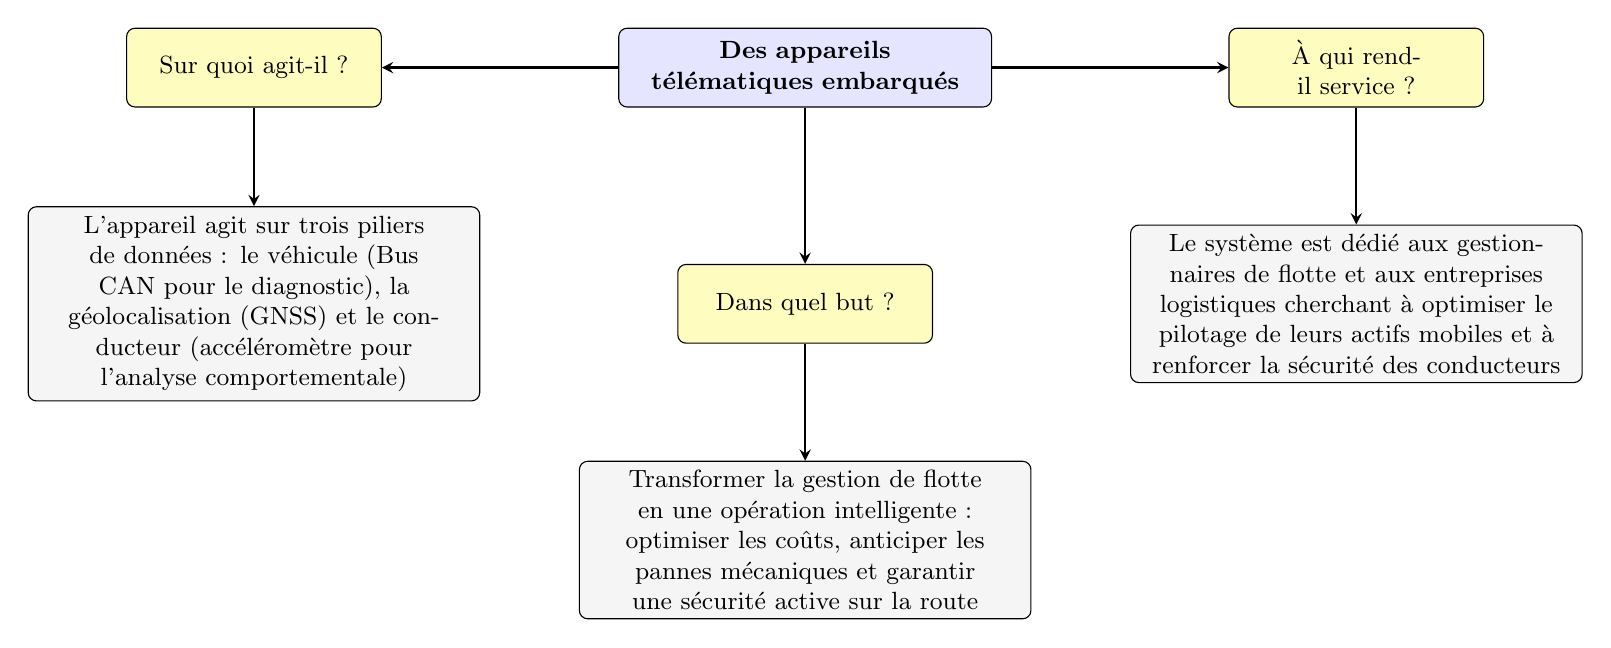
\begin{tikzpicture}[font=\small,
  box/.style={draw, rounded corners=3pt, align=center,
               minimum height=1cm, fill=#1},
  arr/.style={->, thick, >=stealth}
]
  \node[box=blue!10, text width=4.5cm] (center) at (0,0)
        {\textbf{Des appareils télématiques embarqués}};

  \node[box=yellow!25, text width=3cm] (qsujet) at (-7,0)
        {Sur quoi agit-il ?};
  \node[box=yellow!25, text width=3cm] (qcible) at (7,0)
        {À qui rend-il service ?};
  \node[box=yellow!25, text width=3cm] (qbut) at (0,-3)
        {Dans quel but ?};

  \node[box=gray!8, text width=5.5cm] (rsujet) at (-7,-3)
        {L'appareil agit sur trois piliers de données : le véhicule
         (Bus CAN pour le diagnostic), la géolocalisation (GNSS) et
         le conducteur (accéléromètre pour l'analyse
         comportementale)};
  \node[box=gray!8, text width=5.5cm] (rbut) at (0,-6)
        {Transformer la gestion de flotte en une opération
         intelligente : optimiser les coûts, anticiper les pannes
         mécaniques et garantir une sécurité active sur la route};
  \node[box=gray!8, text width=5.5cm] (rcible) at (7,-3)
        {Le système est dédié aux gestionnaires de flotte et aux
         entreprises logistiques cherchant à optimiser le pilotage
         de leurs actifs mobiles et à renforcer la sécurité des
         conducteurs};

  \draw[arr] (center) -- (qsujet);
  \draw[arr] (center) -- (qcible);
  \draw[arr] (center) -- (qbut);
  \draw[arr] (qsujet) -- (rsujet);
  \draw[arr] (qcible) -- (rcible);
  \draw[arr] (qbut)   -- (rbut);
\end{tikzpicture}}
\caption{Diagramme Bête à corne — positionnement fonctionnel initial
         du système \textit{GlobalFleet}}
\label{fig:bete_a_corne}
\end{figure}

%------------------------------------------------------------
% FIGURE 2 : DIAGRAMME PIEUVRE
%------------------------------------------------------------
\begin{figure}[H]
\centering
\resizebox{\textwidth}{!}{%
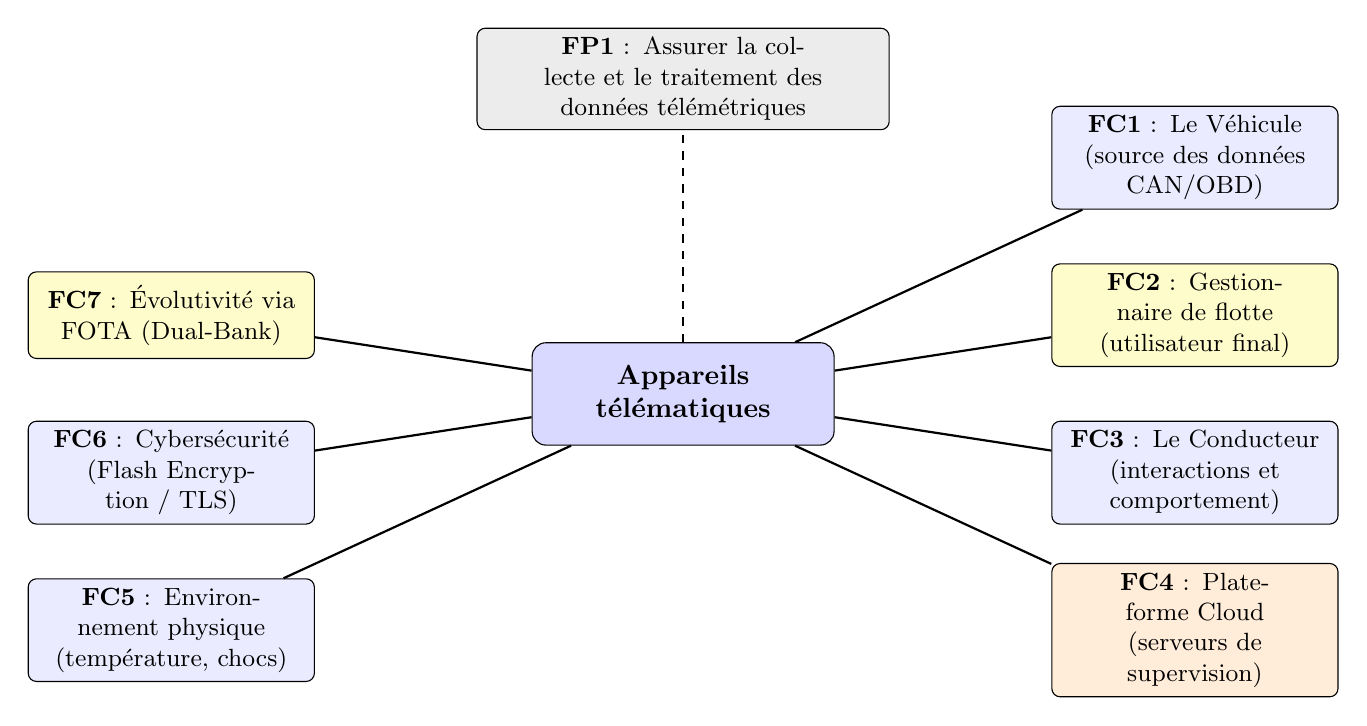
\begin{tikzpicture}[font=\small,
  fc/.style={draw, rounded corners=3pt, align=center,
             text width=3.4cm, minimum height=1.1cm, fill=#1},
  core/.style={draw, rounded corners=5pt, align=center,
               text width=3.6cm, minimum height=1.3cm,
               fill=blue!15, font=\bfseries},
  fp/.style={draw, rounded corners=3pt, align=center,
             text width=5cm, fill=gray!15},
  arr/.style={-, thick}
]
  \node[core] (core) at (0,0) {Appareils\\télématiques};

  \node[fc=blue!8]   (fc1) at (6.5, 3)   {\textbf{FC1} : Le Véhicule\\(source des données CAN/OBD)};
  \node[fc=yellow!20](fc2) at (6.5, 1)   {\textbf{FC2} : Gestionnaire de flotte\\(utilisateur final)};
  \node[fc=blue!8]   (fc3) at (6.5,-1)   {\textbf{FC3} : Le Conducteur\\(interactions et comportement)};
  \node[fc=orange!15](fc4) at (6.5,-3)   {\textbf{FC4} : Plateforme Cloud\\(serveurs de supervision)};

  \node[fc=blue!8]   (fc5) at (-6.5,-3)  {\textbf{FC5} : Environnement physique\\(température, chocs)};
  \node[fc=blue!8]   (fc6) at (-6.5,-1)  {\textbf{FC6} : Cybersécurité\\(Flash Encryption / TLS)};
  \node[fc=yellow!20](fc7) at (-6.5, 1)  {\textbf{FC7} : Évolutivité via\\FOTA (Dual-Bank)};

  \node[fp] (fp1) at (0,4)
        {\textbf{FP1} : Assurer la collecte et le traitement des
         données télémétriques};

  \draw[arr] (core) -- (fc1);
  \draw[arr] (core) -- (fc2);
  \draw[arr] (core) -- (fc3);
  \draw[arr] (core) -- (fc4);
  \draw[arr] (core) -- (fc5);
  \draw[arr] (core) -- (fc6);
  \draw[arr] (core) -- (fc7);
  \draw[arr, dashed] (core) -- (fp1);
\end{tikzpicture}}
\caption{Diagramme Pieuvre — fonction principale (FP1) et contraintes
         fonctionnelles (FC1–FC7) du système \textit{GlobalFleet}}
\label{fig:pieuvre}
\end{figure}

%------------------------------------------------------------
% TABLEAU DES FONCTIONS DE SERVICE
%------------------------------------------------------------
\begin{table}[H]
\centering
\renewcommand{\arraystretch}{1.4}
\caption{Cahier des charges fonctionnel — fonctions de service et
         critères d'évaluation}
\label{tab:fonctions_service}
\small
\begin{tabular}{|c|p{5.5cm}|p{5cm}|}
\hline
\rowcolor{gray!20}
\textbf{Fonction} & \textbf{Description technique} & \textbf{Critère d'évaluation} \\
\hline
FP1 & Traitement des flux CAN \& GNSS & Latence $<$ 100\,ms \\
\hline
FC1 & Interfaçage avec l'ECU du véhicule & Protocole ISO 15765-4 \\
\hline
FC2 & Interface homme-machine (Dashboard) & Temps de réponse $<$ 2\,s \\
\hline
FC3 & Monitoring du style de conduite & Algorithme 3 axes \\
\hline
FC4 & Transmission des données vers le Cloud & Protocole MQTT sécurisé \\
\hline
FC5 & Résistance aux conditions extrêmes & Norme ISO 16750 \\
\hline
FC6 & Protection du firmware & Secure Boot \& Flash Encryption \\
\hline
FC7 & Mise à jour firmware à distance & Mode Dual-Bank (Safe FOTA) \\
\hline
\end{tabular}
\end{table}

%------------------------------------------------------------
% FIGURE 3 : DIAGRAMME FAST
%------------------------------------------------------------
\begin{figure}[H]
\centering
\resizebox{\textwidth}{!}{%
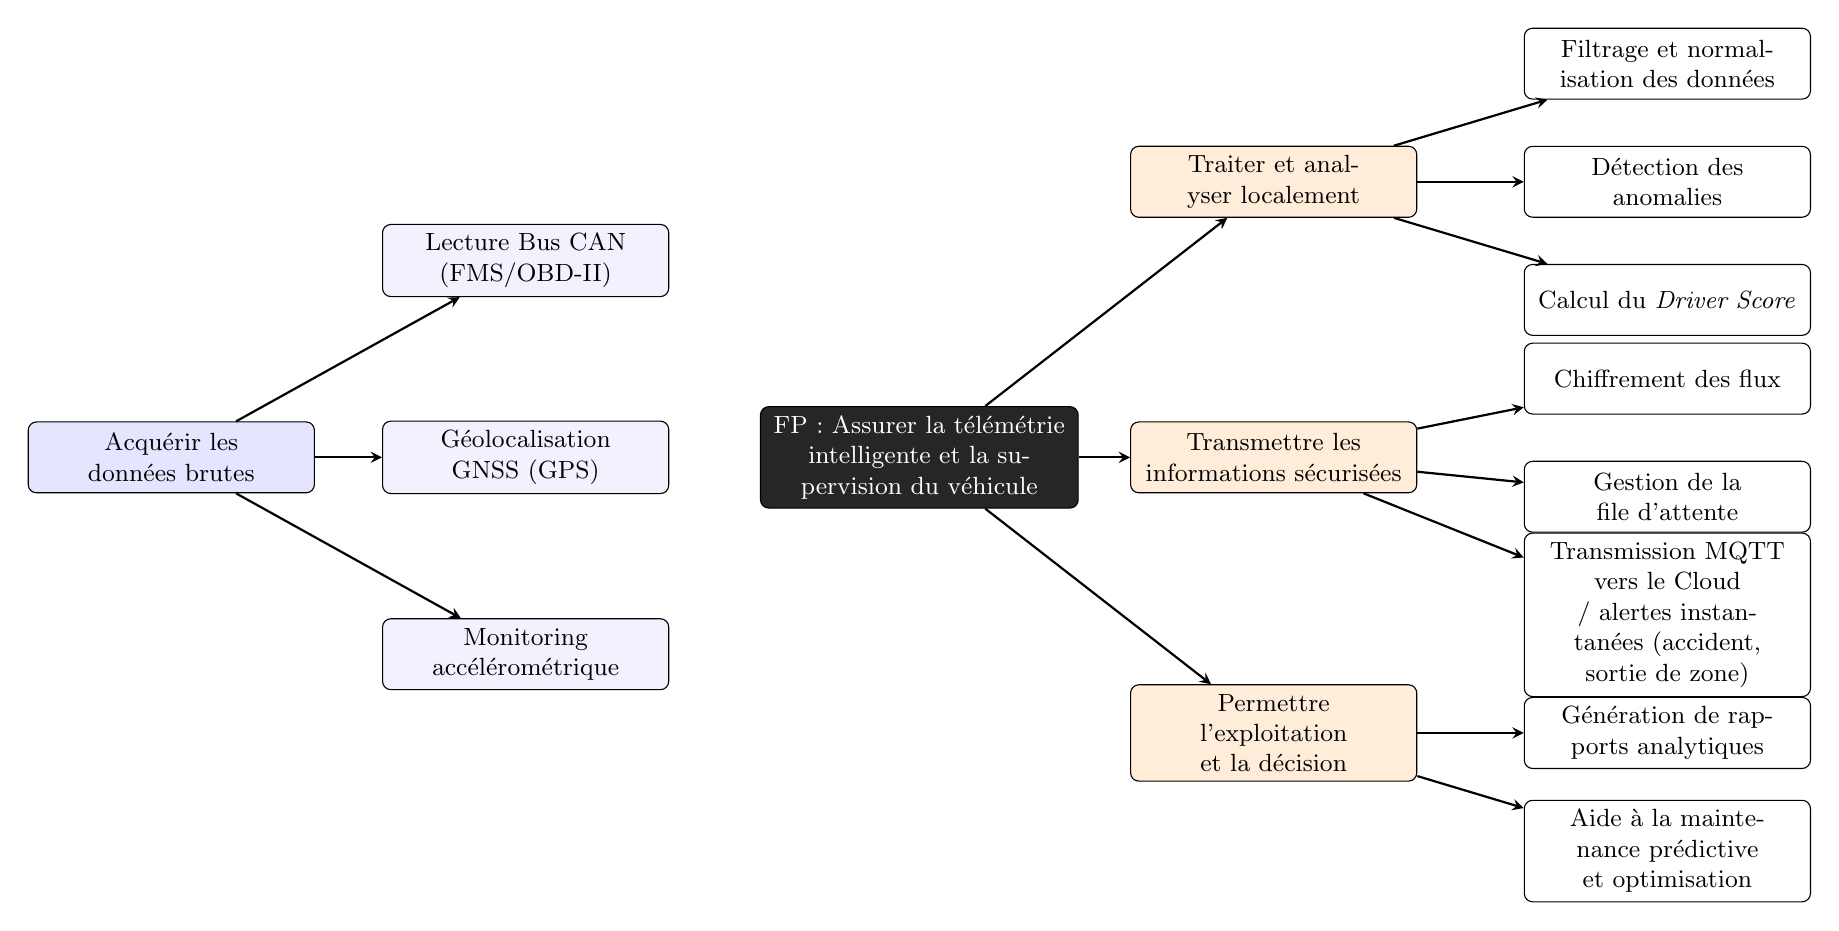
\begin{tikzpicture}[font=\small,
  box/.style={draw, rounded corners=3pt, align=center,
              text width=3.4cm, minimum height=0.9cm, fill=#1},
  arr/.style={->, thick, >=stealth}
]
  % --- Acquisition (gauche) ---
  \node[box=blue!10] (acq) at (0,-1.5) {Acquérir les données brutes};

  \node[box=blue!5] (can) at (4.5, 1)   {Lecture Bus CAN\\(FMS/OBD-II)};
  \node[box=blue!5] (gps) at (4.5,-1.5) {Géolocalisation GNSS (GPS)};
  \node[box=blue!5] (acc) at (4.5,-4)   {Monitoring accélérométrique};

  \draw[arr] (acq) -- (can);
  \draw[arr] (acq) -- (gps);
  \draw[arr] (acq) -- (acc);

  % --- Fonction principale (centre) ---
  \node[box=black!85, text=white, text width=3.8cm] (fp) at (9.5,-1.5)
        {FP : Assurer la télémétrie intelligente et la supervision
         du véhicule};

  % --- Branches principales (droite) ---
  \node[box=orange!15] (traiter)     at (14, 2)   {Traiter et analyser localement};
  \node[box=orange!15] (transmettre) at (14,-1.5) {Transmettre les informations sécurisées};
  \node[box=orange!15] (exploiter)   at (14,-5)   {Permettre l'exploitation et la décision};

  \draw[arr] (fp) -- (traiter);
  \draw[arr] (fp) -- (transmettre);
  \draw[arr] (fp) -- (exploiter);

  % --- Sous-fonctions : Traiter et analyser localement ---
  \node[box=white] (filtrage) at (19, 3.5) {Filtrage et normalisation des données};
  \node[box=white] (anomalie) at (19, 2)   {Détection des anomalies};
  \node[box=white] (score)    at (19, 0.5) {Calcul du \textit{Driver Score}};
  \draw[arr] (traiter) -- (filtrage);
  \draw[arr] (traiter) -- (anomalie);
  \draw[arr] (traiter) -- (score);

  % --- Sous-fonctions : Transmettre les informations sécurisées ---
  \node[box=white] (chiffrement) at (19,-0.5) {Chiffrement des flux};
  \node[box=white] (queue)       at (19,-2)   {Gestion de la file d'attente};
  \node[box=white] (mqtt)        at (19,-3.5) {Transmission MQTT vers le Cloud\\/ alertes instantanées (accident, sortie de zone)};
  \draw[arr] (transmettre) -- (chiffrement);
  \draw[arr] (transmettre) -- (queue);
  \draw[arr] (transmettre) -- (mqtt);

  % --- Sous-fonctions : Permettre l'exploitation et la décision ---
  \node[box=white] (rapport)     at (19,-5)   {Génération de rapports analytiques};
  \node[box=white] (maintenance) at (19,-6.5) {Aide à la maintenance prédictive et optimisation};
  \draw[arr] (exploiter) -- (rapport);
  \draw[arr] (exploiter) -- (maintenance);
\end{tikzpicture}}
\caption{Diagramme FAST — décomposition fonctionnelle du système
         \textit{GlobalFleet}}
\label{fig:fast}
\end{figure}

\newpage

%------------------------------------------------------------
\subsection{Besoin fonctionnel général}
\label{subsec:besoin_fonc}
%------------------------------------------------------------

Le firmware \textit{GlobalFleet} doit assurer la collecte, le
traitement et la transmission de données télémétriques issues de
véhicules équipés de dispositifs embarqués basés sur l'ESP32-P4. Il
supervise en continu l'état du système, gère l'alimentation selon la
dynamique véhicule, enregistre les événements dans un stockage non
volatile et communique avec un serveur distant selon différents
protocoles configurables (MQTT, TCP, UDP). Ces fonctions doivent
opérer de manière fiable dans des environnements contraints :
ressources mémoire limitées, alimentation sur batterie ou sur le
réseau électrique du véhicule, et connectivité cellulaire
intermittente dans les zones à couverture partielle.

L'architecture de traitement suit une logique en pipeline
événementiel : les données brutes sont acquises par les drivers de
périphériques regroupés dans le composant \texttt{hal\_driver} (GPIO,
UART) et dans les composants spécialisés (\texttt{can\_driver},
\texttt{gps}, \texttt{sensors}), puis normalisées et publiées sur
le bus d'événements interne implémenté dans le composant
\texttt{event\_bus}. Les modules consommateurs abonnés via le
\texttt{subscription\_manager} récupèrent les événements typés pour
les traiter, les stocker localement via \texttt{storage\_api}, ou
les transmettre vers le cloud via \texttt{comms\_manager}. Cette
organisation pipeline garantit que l'ajout d'une nouvelle source de
données n'impose aucune modification aux composants de traitement
existants, réduisant le risque de régression lors de l'évolution
de la gamme matérielle SAT.

\begin{figure}[H]
\centering
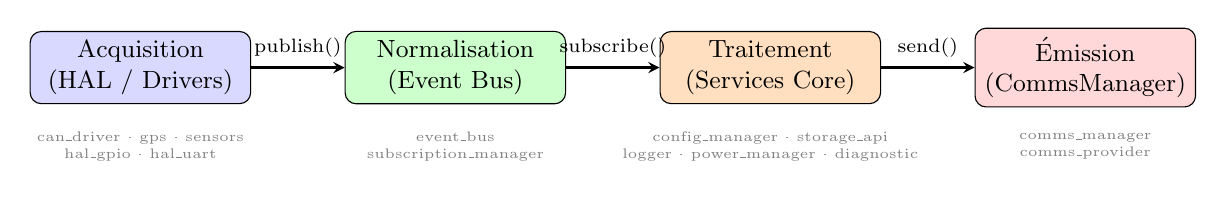
\begin{tikzpicture}[font=\small,
  stage/.style={draw, rounded corners=4pt, minimum width=2.8cm,
                minimum height=0.9cm, align=center, fill=#1},
  arr/.style={->, thick, >=stealth}
]
  \node[stage=blue!15]   (acq)   at (0,0)    {Acquisition\\(HAL / Drivers)};
  \node[stage=green!20]  (norm)  at (4,0)    {Normalisation\\(Event Bus)};
  \node[stage=orange!25] (proc)  at (8,0)    {Traitement\\(Services Core)};
  \node[stage=red!15]    (emit)  at (12,0)   {Émission\\(CommsManager)};
  \draw[arr] (acq)  -- node[above]{\scriptsize publish()} (norm);
  \draw[arr] (norm) -- node[above]{\scriptsize subscribe()} (proc);
  \draw[arr] (proc) -- node[above]{\scriptsize send()} (emit);
  % sous-composants
  \node[font=\tiny, gray, align=center] at (0,-1.0)
        {can\_driver · gps · sensors\\hal\_gpio · hal\_uart};
  \node[font=\tiny, gray, align=center] at (4,-1.0)
        {event\_bus\\subscription\_manager};
  \node[font=\tiny, gray, align=center] at (8,-1.0)
        {config\_manager · storage\_api\\logger · power\_manager · diagnostic};
  \node[font=\tiny, gray, align=center] at (12,-1.0)
        {comms\_manager\\comms\_provider};
\end{tikzpicture}
\caption{Pipeline événementiel du firmware \textit{GlobalFleet} — des drivers jusqu'à l'émission cloud}
\label{fig:pipeline}
\end{figure}

%------------------------------------------------------------
\subsection{Besoin de généricité}
\label{subsec:besoin_gen}
%------------------------------------------------------------

La gamme SAT couvre plusieurs variantes matérielles — \textbf{Basic},
\textbf{Pro} et \textbf{Ultra-Pro} — qui diffèrent par leurs
périphériques embarqués : présence ou absence du module GNSS
(\texttt{gps}), du bus CAN (\texttt{can\_driver}), de capteurs
additionnels (\texttt{sensors}), du module Secure Boot
(\texttt{secure\_boot}), et de capacités de chiffrement Flash. Le
firmware doit fonctionner sur l'ensemble de ces variantes à partir
d'une seule base de code unifiée, sans recompilation conditionnelle
proliférante qui fragmenterait la maintenance et compliquerait les
campagnes de tests. La différenciation entre variantes repose sur
deux mécanismes complémentaires : des options de compilation gérées
via le système \texttt{Kconfig} d'ESP-IDF (fichier
\texttt{Kconfig.projbuild} visible à la racine du composant
\texttt{main}), et un registre de capacités persisté en NVS
paramétrant le comportement à l'exécution. Ce double mécanisme
permet de distribuer le même binaire à l'ensemble de la flotte et
de configurer le profil fonctionnel de chaque appareil lors de
la programmation usine, sans intervention logicielle ultérieure.
Le registre est ensuite interrogé dynamiquement par chaque
composant au démarrage via la macro \texttt{HAS\_CAPABILITY(reg, bit)},
garantissant que les ressources non disponibles ne sont jamais
initialisées, ce qui élimine les erreurs d'accès à des périphériques
absents tout en préservant l'intégrité du binaire commun.

%------------------------------------------------------------
\subsection{Besoin de modularité}
\label{subsec:besoin_mod}
%------------------------------------------------------------

Chaque service fonctionnel du firmware est encapsulé dans un composant
ESP-IDF indépendant, disposant de son propre répertoire, de ses
fichiers sources \texttt{.c}/\texttt{.h} et de son fichier
\texttt{CMakeLists.txt} déclarant ses dépendances. Cette organisation,
visible dans la structure \texttt{components/} du dépôt, regroupe
vingt-trois composants distincts : \texttt{can\_driver},
\texttt{comms\_manager}, \texttt{comms\_provider},
\texttt{config\_manager}, \texttt{diagnostic}, \texttt{error\_manager},
\texttt{event\_bus}, \texttt{fault\_manager}, \texttt{gps},
\texttt{hal\_driver}, \texttt{logger}, \texttt{module\_health},
\texttt{module\_interface}, \texttt{ota\_manager},
\texttt{power\_manager}, \texttt{ring\_buffer}, \texttt{secure\_boot},
\texttt{sensors}, \texttt{serial\_comm}, \texttt{storage\_api},
\texttt{subscription\_manager} et \texttt{watchdog\_task}. Ce
découplage producteur-consommateur, réalisé via le bus d'événements,
garantit que l'ajout d'un nouveau module de traitement n'impose aucune
modification aux composants existants. Chaque module expose
l'interface standardisée \texttt{module\_interface\_t} définie dans
le composant \texttt{module\_interface}, ce qui rend tous les
composants manipulables de façon uniforme par le gestionnaire de
cycle de vie du noyau. Cette exigence facilite les tests unitaires
par isolation de composant, le remplacement d'une implémentation par
une alternative, et l'intégration de nouveaux services sans
refactorisation globale de la base de code.

\begin{figure}[H]
\centering
\begin{tikzpicture}[font=\scriptsize,
  comp/.style={draw, rounded corners=3pt, minimum width=2.6cm,
               minimum height=0.55cm, align=center, fill=#1},
  grp/.style={draw=gray!50, dashed, rounded corners=5pt, inner sep=6pt}
]
  % Groupe HAL
  \begin{scope}
  \node[comp=orange!20] (hgpio) at (0,0)    {hal\_gpio};
  \node[comp=orange!20] (huart) at (0,-0.8) {hal\_uart};
  \node[comp=orange!20] (cand)  at (0,-1.6) {can\_driver};
  \node[comp=orange!20] (gpsd)  at (0,-2.4) {gps};
  \node[comp=orange!20] (sens)  at (0,-3.2) {sensors};
  \node[grp, fit=(hgpio)(huart)(cand)(gpsd)(sens)] (ghal) {};
  \node[font=\tiny\bfseries, gray] at (0, 0.55) {HAL \& Drivers};
  \end{scope}
  % Groupe Noyau
  \begin{scope}
  \node[comp=green!20] (ebus)  at (4.2, 0)    {event\_bus};
  \node[comp=green!20] (subm)  at (4.2,-0.8)  {subscription\_manager};
  \node[comp=green!20] (wdt)   at (4.2,-1.6)  {watchdog\_task};
  \node[comp=green!20] (mh)    at (4.2,-2.4)  {module\_health};
  \node[comp=green!20] (mi)    at (4.2,-3.2)  {module\_interface};
  \node[grp, fit=(ebus)(subm)(wdt)(mh)(mi)] (gnoyau) {};
  \node[font=\tiny\bfseries, gray] at (4.2, 0.55) {Noyau RTOS};
  \end{scope}
  % Groupe Services
  \begin{scope}
  \node[comp=blue!15] (cfg)  at (8.4, 0)    {config\_manager};
  \node[comp=blue!15] (sto)  at (8.4,-0.8)  {storage\_api};
  \node[comp=blue!15] (log)  at (8.4,-1.6)  {logger};
  \node[comp=blue!15] (pw)   at (8.4,-2.4)  {power\_manager};
  \node[comp=blue!15] (dia)  at (8.4,-3.2)  {diagnostic};
  \node[comp=blue!15] (err)  at (8.4,-4.0)  {error\_manager};
  \node[grp, fit=(cfg)(sto)(log)(pw)(dia)(err)] (gsvc) {};
  \node[font=\tiny\bfseries, gray] at (8.4, 0.55) {Services Core};
  \end{scope}
  % Groupe Applicatif
  \begin{scope}
  \node[comp=red!15]  (cm)  at (12.6, 0)    {comms\_manager};
  \node[comp=red!15]  (cp)  at (12.6,-0.8)  {comms\_provider};
  \node[comp=red!15]  (ota) at (12.6,-1.6)  {ota\_manager};
  \node[comp=red!15]  (fm)  at (12.6,-2.4)  {fault\_manager};
  \node[comp=red!15]  (sc)  at (12.6,-3.2)  {serial\_comm};
  \node[comp=red!15]  (sb)  at (12.6,-4.0)  {secure\_boot};
  \node[grp, fit=(cm)(cp)(ota)(fm)(sc)(sb)] (gapp) {};
  \node[font=\tiny\bfseries, gray] at (12.6, 0.55) {Applicatif};
  \end{scope}
  % Flèches inter-groupes
  \draw[->, thick, >=stealth] (ghal.east)   -- (gnoyau.west);
  \draw[->, thick, >=stealth] (gnoyau.east) -- (gsvc.west);
  \draw[->, thick, >=stealth] (gsvc.east)   -- (gapp.west);
\end{tikzpicture}
\caption{Décomposition modulaire du projet \textit{GlobalFleet} en 23 composants ESP-IDF}
\label{fig:decomp_modulaire}
\end{figure}

%------------------------------------------------------------
\subsection{Besoin de configurabilité}
\label{subsec:besoin_config}
%------------------------------------------------------------

Le comportement du firmware doit être ajustable sans recompilation,
tant en usine (paramètres matériels fixes) que sur le terrain
(paramètres opérationnels : intervalles de rapport, seuils d'alerte,
protocole de communication actif, politique de veille). Cette exigence
est satisfaite par le composant \texttt{config\_manager}, qui gère
deux espaces NVS distincts : \texttt{nvs\_factory} pour les paramètres
de fabrication immuables (numéro de série, type de matériel, valeur
du registre de capacités) et \texttt{nvs\_field} pour les paramètres
terrain modifiables à distance (APN cellulaire, broker MQTT, intervalles
de reporting, seuils de détection). Chaque bloc de configuration field
embarque un numéro de version sur 16~bits et un CRC-32 calculé sur
l'ensemble des champs. Au démarrage, \texttt{config\_manager} vérifie
l'intégrité du CRC et compare le numéro de version avec la version
attendue par le firmware courant. En cas de discordance, la procédure
de repli est déclenchée automatiquement : le firmware charge une
structure \textit{hardcoded defaults} codée en dur et expose un
indicateur \texttt{config\_fallback\_active} au module
\texttt{diagnostic} pour signalement vers le serveur. Ce mécanisme
garantit qu'un appareil déployé en conditions réelles ne reste jamais
bloqué sur une configuration corrompue, et que toute intervention de
maintenance peut s'effectuer à distance sans accès physique à l'appareil.

%------------------------------------------------------------
\subsection{Besoin de fiabilité et de diagnostic}
\label{subsec:besoin_fiab}
%------------------------------------------------------------

Un appareil télématique déployé en flotte doit être capable
d'auto-diagnostiquer ses propres défaillances et d'appliquer des
stratégies de récupération graduées sans intervention humaine.
Le firmware \textit{GlobalFleet} répond à cette exigence par une
architecture de supervision à trois niveaux, incarnée par les
composants \texttt{watchdog\_task}, \texttt{module\_health} et
\texttt{fault\_manager}. Le composant \texttt{watchdog\_task}
surveille en permanence les heartbeats de chaque tâche FreeRTOS et
publie un événement \texttt{EVT\_WDT\_TIMEOUT} sur le bus dès qu'une
tâche devient silencieuse au-delà du délai configuré. Le composant
\texttt{module\_health} maintient des compteurs de santé individuels
par module, incrémentés à chaque anomalie et décrémentés
périodiquement pour détecter les dégradations progressives avant
qu'elles ne deviennent critiques. Le composant \texttt{fault\_manager}
centralise la classification des fautes selon quatre niveaux de
sévérité (WARNING, ERROR, CRITICAL, FATAL) et applique la politique
de récupération correspondante. En mode FATAL, il capture un snapshot
complet de diagnostic en NVS et le transmet au serveur lors du
rétablissement de la connectivité, permettant un diagnostic post-mortem
précis sans accès physique à l'appareil. Cette approche garantit la
continuité de service même face à des défaillances partielles de
composants, tout en évitant les redémarrages intempestifs qui
dégraderaient la qualité de service des appareils en flotte.

%------------------------------------------------------------
\subsection{Besoin d'intégration avec les autres axes du projet}
\label{subsec:besoin_integ}
%------------------------------------------------------------

Le firmware constitue l'un des axes d'un projet plus large incluant
une application mobile, un serveur de gestion de flotte et une
infrastructure cloud. Il doit donc exposer des interfaces de
communication standardisées et interopérables avec les autres
composants du système. Le composant \texttt{comms\_provider} définit
une interface C abstraite supportant MQTT TLS~1.3, TCP et UDP,
sélectionnée à l'exécution par le \texttt{comms\_manager} selon
la configuration terrain. Le composant \texttt{ota\_manager}
implémente le mécanisme FOTA Dual-Bank permettant les mises à jour
à distance sécurisées avec rollback automatique, assurant la
continuité de service lors des montées de version. Le composant
\texttt{secure\_boot} s'inscrit dans la chaîne de sécurité globale
du projet, garantissant l'intégrité du code exécuté via le mécanisme
ESP32 Secure Boot v2 et Flash Encryption activé pour la variante
Ultra-Pro. Le composant \texttt{serial\_comm} assure la communication
locale par port série pour la configuration de premier démarrage et
le diagnostic sur le terrain. Enfin, le composant \texttt{diagnostic}
expose en permanence les métriques système (raison du dernier
redémarrage, uptime, health counters, utilisation mémoire, statistiques
réseau) au format structuré JSON, directement consommable par le
serveur de gestion de flotte de SAT, garantissant la cohérence de
l'interface entre les axes du projet.

%============================================================
\section{Modèle de capacités et modèle de configuration}
\label{sec:capabilities}
%============================================================

%------------------------------------------------------------
\subsection{Capabilities model : description des fonctionnalités
hardware disponibles}
\label{subsec:cap_model}
%------------------------------------------------------------

Le modèle de capacités est la réponse architecturale centrale au
problème de généricité multi-variante : il s'agit d'un mécanisme
déclaratif permettant d'activer ou de désactiver des groupes de
fonctionnalités par simple reconfiguration d'un registre NVS, sans
toucher au code source ni relancer une compilation. Il est implémenté
sous la forme d'un registre de 32~bits persisté dans la partition NVS
factory sous la clé \texttt{capabilities\_register}, dans lequel
chaque bit correspond à une fonctionnalité optionnelle. Ce registre
est initialisé lors de la programmation usine selon le profil de la
variante, et lu au démarrage par le composant \texttt{config\_manager}
avant toute initialisation de périphérique. La macro
\texttt{HAS\_CAPABILITY(reg, bit)} permet à chaque composant de tester
dynamiquement la présence d'une fonctionnalité : le composant
\texttt{can\_driver} vérifie le bit~1 avant d'initialiser le
contrôleur TWAI, le composant \texttt{gps} vérifie le bit~0 avant de
démarrer la tâche GNSS, et ainsi de suite pour chaque périphérique
optionnel. Ce mécanisme élimine les directives de compilation
conditionnelle dans le code applicatif et centralise toute la logique
de différenciation dans un registre unique, versifiable et auditable.
Le tableau~\ref{tab:variantes} présente la répartition des capacités
pour les trois variantes de la gamme SAT.

\begin{figure}[H]
    \centering
    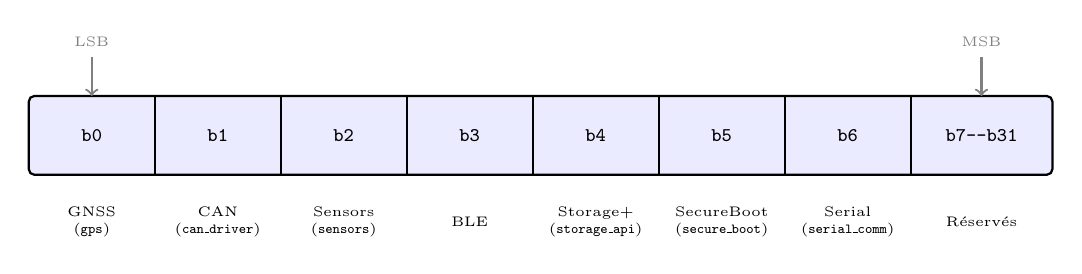
\begin{tikzpicture}[font=\small]
      % Registre 32 bits
      \draw[thick, rounded corners=2pt, fill=blue!8]
            (0,0) rectangle (13,1.0);
      % séparateurs
      \foreach \x in {1.6,3.2,4.8,6.4,8.0,9.6,11.2} {
        \draw[thick] (\x,0) -- (\x,1.0);
      }
      % labels bits
      \node[font=\bfseries\scriptsize] at (0.8, 0.5)  {\texttt{b0}};
      \node[font=\bfseries\scriptsize] at (2.4, 0.5)  {\texttt{b1}};
      \node[font=\bfseries\scriptsize] at (4.0, 0.5)  {\texttt{b2}};
      \node[font=\bfseries\scriptsize] at (5.6, 0.5)  {\texttt{b3}};
      \node[font=\bfseries\scriptsize] at (7.2, 0.5)  {\texttt{b4}};
      \node[font=\bfseries\scriptsize] at (8.8, 0.5)  {\texttt{b5}};
      \node[font=\bfseries\scriptsize] at (10.4,0.5)  {\texttt{b6}};
      \node[font=\bfseries\scriptsize] at (12.1,0.5)  {\texttt{b7--b31}};
      % étiquettes fonctionnalités
      \node[font=\tiny, align=center] at (0.8, -0.6)  {GNSS\\(\texttt{gps})};
      \node[font=\tiny, align=center] at (2.4, -0.6)  {CAN\\(\texttt{can\_driver})};
      \node[font=\tiny, align=center] at (4.0, -0.6)  {Sensors\\(\texttt{sensors})};
      \node[font=\tiny, align=center] at (5.6, -0.6)  {BLE};
      \node[font=\tiny, align=center] at (7.2, -0.6)  {Storage+\\(\texttt{storage\_api})};
      \node[font=\tiny, align=center] at (8.8, -0.6)  {SecureBoot\\(\texttt{secure\_boot})};
      \node[font=\tiny, align=center] at (10.4,-0.6)  {Serial\\(\texttt{serial\_comm})};
      \node[font=\tiny, align=center] at (12.1,-0.6)  {Réservés};
      % flèche annotation
      \draw[<-, gray, thick] (0.8,1.0) -- ++(0,0.5)
            node[above, font=\tiny]{LSB};
      \draw[<-, gray, thick] (12.1,1.0) -- ++(0,0.5)
            node[above, font=\tiny]{MSB};
    \end{tikzpicture}
    \caption{Structure du registre de capacités 32~bits — chaque bit active un composant ESP-IDF}
    \label{fig:capabilities_register}
\end{figure}
La figure~\ref{fig:capabilities_register} illustre la correspondance
entre chaque bit du registre et le composant ESP-IDF qu'il contrôle :
les bits~0 à~6 activent respectivement les composants \texttt{gps},
\texttt{can\_driver}, \texttt{sensors}, le module BLE,
\texttt{storage\_api} (mode étendu), \texttt{secure\_boot} et
\texttt{serial\_comm}, tandis que les bits~7 à~31 sont réservés pour
de futures extensions matérielles sans qu'aucune modification du
format de configuration ne soit nécessaire. À la programmation usine,
ce registre est positionné selon la variante commandée — \textbf{Basic},
\textbf{Pro} ou \textbf{Ultra-Pro} — chacune correspondant à un profil
de bits prédéfini correspondant à un sous-ensemble croissant de
fonctionnalités
\newpage
Le tableau~\ref{tab:variantes} détaille, pour chaque
variante, l'ensemble des fonctionnalités activées et le composant
logiciel associé.
\begin{table}[H]
\centering
\renewcommand{\arraystretch}{1.6}
\caption{Capacités activées par variante de produit SAT}
\label{tab:variantes}
\footnotesize
\begin{tabular}{|p{5.5cm}|c|c|c|c|}
\hline
\rowcolor{gray!20}
\textbf{Fonctionnalité} & \textbf{Composant} &
\textbf{Basic} & \textbf{Pro} & \textbf{Ultra-Pro} \\
\hline
Localisation GNSS multi-constellation & \texttt{gps}
  & \checkmark & \checkmark & \checkmark \\
\hline
Transmission cellulaire LTE Cat-M1    & \texttt{comms\_manager}
  & \checkmark & \checkmark & \checkmark \\
\hline
Stockage local / file persistante     & \texttt{storage\_api}
  & \checkmark & \checkmark & \checkmark \\
\hline
Gestion d'énergie basse consommation  & \texttt{power\_manager}
  & \checkmark & \checkmark & \checkmark \\
\hline
Journalisation et diagnostic système  & \texttt{logger}, \texttt{diagnostic}
  & \checkmark & \checkmark & \checkmark \\
\hline
Communication locale série            & \texttt{serial\_comm}
  & \checkmark & \checkmark & \checkmark \\
\hline
Lecture Bus CAN (OBD-II / J1939)      & \texttt{can\_driver}
  &            & \checkmark & \checkmark \\
\hline
Capteurs additionnels                 & \texttt{sensors}
  &            & \checkmark & \checkmark \\
\hline
Transmission MQTT sécurisée TLS~1.3   & \texttt{comms\_provider}
  &            & \checkmark & \checkmark \\
\hline
FOTA Dual-Bank sécurisé               & \texttt{ota\_manager}
  &            &            & \checkmark \\
\hline
Flash Encryption \& Secure Boot v2    & \texttt{secure\_boot}
  &            &            & \checkmark \\
\hline
Ultra-Low Power ($<$\,2\,mA)          & \texttt{power\_manager}
  &            &            & \checkmark \\
\hline
\end{tabular}
\end{table}

%------------------------------------------------------------
\subsection{Config model : choix runtime et paramètres applicatifs}
\label{subsec:config_model}
%------------------------------------------------------------

Le modèle de configuration gère deux niveaux de paramètres distincts,
implémentés dans le composant \texttt{config\_manager}. La
\textbf{configuration factory} regroupe les paramètres de fabrication
écrits une seule fois lors de la programmation en usine : identifiant
unique du dispositif, type de matériel, clés de sécurité TLS, adresse
du serveur de référence, et valeur du registre de capacités. Ces
paramètres sont persistés dans la partition NVS \texttt{nvs\_factory}
et protégés par un drapeau \texttt{factory\_locked} qui empêche toute
écriture accidentelle depuis l'applicatif. En variante Ultra-Pro, la
partition factory est protégée par Flash Encryption activée via le
composant \texttt{secure\_boot}. La \textbf{configuration field}
regroupe les paramètres opérationnels modifiables à distance :
intervalles de rapport périodique, seuils d'alerte (accélération G,
vitesse maximale geofencing), protocole de communication actif (MQTT,
TCP ou UDP sélectionné par le \texttt{comms\_manager}), politique de
veille (\texttt{power\_manager}), topics MQTT, et paramètres APN. Ces
paramètres sont stockés dans la partition \texttt{nvs\_field} avec
versioning 16~bits et CRC-32. L'API \texttt{config\_get()},
\texttt{config\_set()} et \texttt{config\_apply()} expose ces deux
espaces de configuration de façon unifiée aux autres composants, qui
ignorent les détails de persistance NVS sous-jacents.

%------------------------------------------------------------
\subsection{Séparation entre configuration usine et configuration terrain}
\label{subsec:sep_config}
%------------------------------------------------------------

La séparation entre les deux espaces de configuration repose sur
l'organisation des partitions NVS définie dans le fichier
\texttt{partitions.csv} visible à la racine du dépôt. La partition
\texttt{nvs\_factory} est montée en lecture seule depuis l'applicatif
dès lors que le drapeau \texttt{factory\_locked} est positionné lors
de la programmation usine. La partition \texttt{nvs\_field} est montée
en lecture/écriture et constitue l'espace de configuration modifiable
tout au long de la vie de l'appareil. Cette architecture reflète les
pratiques de déploiement industriel où les paramètres de fabrication
ne doivent jamais être altérés après la phase de test en usine, même
en cas de bug applicatif ou de tentative de mise à jour malveillante.
Le composant \texttt{config\_manager} encapsule cette logique de
séparation et présente une API unique aux autres composants, qui
n'ont pas connaissance de la partition sous-jacente utilisée.
La partition \texttt{nvs\_field} est intégralement réinitialisée
lors d'un rollback FOTA via \texttt{ota\_manager} si la version du
firmware cible est incompatible avec la structure de configuration
existante, garantissant la cohérence entre le binaire exécuté et
les paramètres persistés.

%------------------------------------------------------------
\subsection{Versioning, CRC et validation de configuration}
\label{subsec:versioning}
%------------------------------------------------------------

Chaque bloc de configuration field persisté en NVS embarque deux
métadonnées d'intégrité : un numéro de version sur 16~bits et un
CRC-32 calculé sur l'ensemble des champs du bloc. Au démarrage, le
composant \texttt{config\_manager} effectue deux vérifications
successives avant toute utilisation des paramètres : il recalcule
le CRC-32 sur les données lues et le compare à la valeur persistée,
puis il compare le numéro de version avec la version attendue par le
firmware courant compilée en dur dans le binaire. Si l'une ou l'autre
des vérifications échoue — qu'il s'agisse d'une corruption flash,
d'une coupure d'alimentation lors d'une écriture, ou d'une mise à
jour de firmware incompatible — la procédure de repli est déclenchée
automatiquement sans blocage du démarrage. Ce mécanisme à double
vérification est essentiel pour des appareils déployés en conditions
réelles où la fiabilité du stockage flash peut être compromise par
des chocs, des variations de température ou des coupures d'alimentation
intempestives lors des transports. La figure~\ref{fig:config_module}
illustre l'enchaînement de ces vérifications au sein du composant
\texttt{config\_manager}.

%------------------------------------------------------------
\subsection{Fallback en cas de configuration invalide}
\label{subsec:fallback}
%------------------------------------------------------------

Lorsque la vérification CRC ou la comparaison de version échoue, le
composant \texttt{config\_manager} charge une structure de
configuration par défaut codée en dur dans le binaire
(\textit{hardcoded defaults}). Ces valeurs par défaut sont
soigneusement dimensionnées pour permettre le fonctionnement minimal
de l'appareil : intervalles de rapport conservateurs, protocole TCP
sans TLS, politique de veille agressive pour économiser la batterie.
Un événement de niveau \texttt{WARN} est immédiatement publié sur
l'event bus, et l'indicateur \texttt{config\_fallback\_active} est
positionné dans la structure d'état du composant \texttt{diagnostic}.
Lors du rétablissement de la connectivité, le composant
\texttt{comms\_manager} transmet automatiquement cet indicateur au
serveur de gestion de flotte, permettant à l'opérateur d'identifier
les appareils en mode dégradé et de déclencher une procédure de
reconfiguration à distance via le canal MQTT. Ce mécanisme garantit
qu'aucun appareil de la flotte ne reste définitivement bloqué sur une
configuration invalide, même sans accès physique possible, ce qui est
critique pour des déploiements géographiquement dispersés.

%============================================================
\section{Machine à états système (FSM)}
\label{sec:fsm}
%============================================================

Un système embarqué déployé en conditions réelles doit gérer des
transitions entre phases opérationnelles distinctes de manière
déterministe et auditable. Implémenter ces transitions sans structure
formelle aboutit systématiquement à un code illisible, difficile à
tester et propice aux états incohérents lors des phases de
récupération après faute. La machine à états finis (FSM) du firmware
\textit{GlobalFleet} rend les cinq états du système explicites, les
transitions déterministes et conditionnées par des événements typés,
et garantit qu'aucune transition non autorisée ne peut survenir. Elle
est pilotée par la \textit{main task} de \texttt{main.c} qui
s'abonne aux événements de transition via le \texttt{subscription\_manager}
et invoque les handlers d'état correspondants. La figure~\ref{fig:fsm_tikz}
illustre les cinq états et l'ensemble des transitions autorisées.

\begin{figure}[H]
\centering
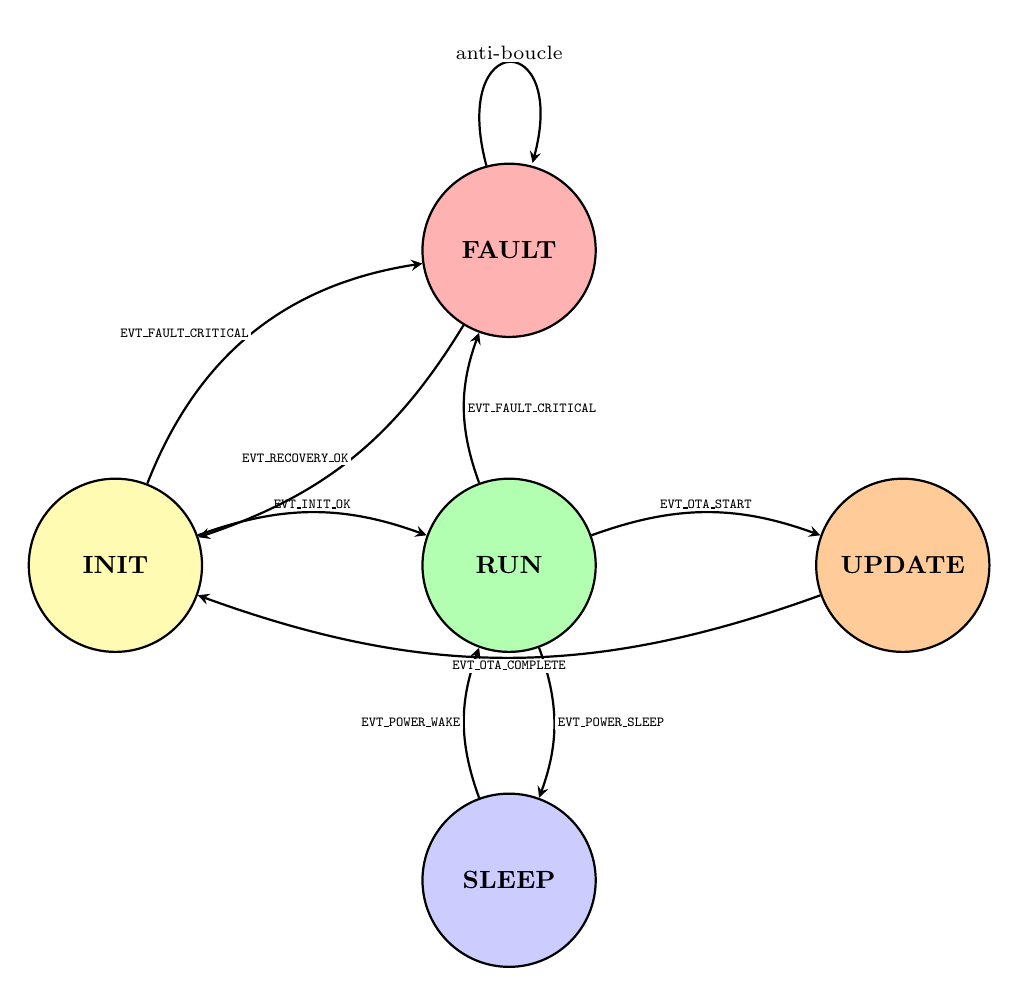
\begin{tikzpicture}[font=\small,
  state/.style={draw, circle, minimum size=2.2cm, align=center,
                thick, fill=#1},
  arr/.style={->, thick, >=stealth, bend left=20},
  label/.style={font=\tiny, fill=white, inner sep=1pt}
]
  % États
  \node[state=yellow!30]  (init)   at (0, 0)     {\textbf{INIT}};
  \node[state=green!30]   (run)    at (5, 0)     {\textbf{RUN}};
  \node[state=blue!20]    (sleep)  at (5,-4)     {\textbf{SLEEP}};
  \node[state=orange!40]  (update) at (10, 0)    {\textbf{UPDATE}};
  \node[state=red!30]     (fault)  at (5, 4)     {\textbf{FAULT}};
  % Transitions
  \draw[arr] (init)   to node[label, above]{\texttt{EVT\_INIT\_OK}} (run);
  \draw[arr] (run)    to node[label, right]{\texttt{EVT\_POWER\_SLEEP}} (sleep);
  \draw[arr] (sleep)  to[bend left=20] node[label, left]{\texttt{EVT\_POWER\_WAKE}} (run);
  \draw[arr] (run)    to node[label, above]{\texttt{EVT\_OTA\_START}} (update);
  \draw[arr] (update) to[bend left=20] node[label, below]{\texttt{EVT\_OTA\_COMPLETE}} (init);
  \draw[arr] (run)    to node[label, right]{\texttt{EVT\_FAULT\_CRITICAL}} (fault);
  \draw[arr] (init)   to[bend left=30] node[label, left]{\texttt{EVT\_FAULT\_CRITICAL}} (fault);
  \draw[arr] (fault)  to node[label, left]{\texttt{EVT\_RECOVERY\_OK}} (init);
  % auto-boucle FAULT
  \draw[->, thick, >=stealth] (fault) edge[loop above]
        node[label]{\scriptsize anti-boucle} (fault);
\end{tikzpicture}
\caption{Machine à états finis du firmware \textit{GlobalFleet} — 5 états, 8 transitions}
\label{fig:fsm_tikz}
\end{figure}

%------------------------------------------------------------
\subsection{État INIT}
\label{subsec:fsm_init}
%------------------------------------------------------------

L'état \texttt{INIT} est l'état initial après tout démarrage ou
redémarrage, qu'il soit provoqué par une mise sous tension, un
watchdog timeout, un retour de l'état \texttt{FAULT} après
récupération, ou un redémarrage post-FOTA depuis l'état
\texttt{UPDATE}. La séquence d'initialisation exécutée dans cet
état suit un ordre strict déterminé par les dépendances entre
composants : le composant \texttt{config\_manager} est initialisé
en premier pour charger le registre de capacités et les paramètres
système, suivi du composant \texttt{hal\_driver} qui initialise
les drivers GPIO et UART selon les capacités détectées, puis des
composants périphériques (\texttt{gps}, \texttt{can\_driver},
\texttt{sensors}) conditionnellement activés par le registre de
capacités, puis du composant \texttt{event\_bus} et du
\texttt{subscription\_manager}, et enfin du \texttt{watchdog\_task}
qui démarre la supervision. Toute erreur fatale durant cette
séquence — échec d'initialisation d'un driver critique, corruption
NVS irrecupérable, allocation mémoire impossible — provoque
immédiatement la transition vers l'état \texttt{FAULT} via
publication de \texttt{EVT\_FAULT\_CRITICAL} sur l'event bus.
En cas de succès complet, l'événement \texttt{EVT\_INIT\_OK} est
publié et le système transite vers l'état \texttt{RUN}.

%------------------------------------------------------------
\subsection{État RUN}
\label{subsec:fsm_run}
%------------------------------------------------------------

L'état \texttt{RUN} correspond au fonctionnement nominal du firmware.
Dans cet état, toutes les tâches FreeRTOS correspondant au profil de
capacités de la variante sont actives et s'exécutent selon leurs
priorités respectives : la tâche de collecte GNSS (\texttt{gps}),
la tâche de lecture CAN (\texttt{can\_driver} si le bit~1 du registre
est positionné), les tâches de communication (\texttt{comms\_manager})
et de stockage (\texttt{storage\_api}). Le composant \texttt{watchdog\_task}
surveille en permanence les heartbeats de chacune de ces tâches et
publie \texttt{EVT\_WDT\_TIMEOUT} si l'une d'elles devient silencieuse.
Le composant \texttt{module\_health} maintient les compteurs de santé
individuels. Trois types de transitions sortantes sont possibles depuis
\texttt{RUN} : vers \texttt{SLEEP} lorsque le \texttt{power\_manager}
détecte une immobilisation prolongée du véhicule et publie
\texttt{EVT\_POWER\_SLEEP} ; vers \texttt{UPDATE} lors de la
réception d'une notification FOTA authentifiée générant
\texttt{EVT\_OTA\_START} ; ou vers \texttt{FAULT} lors d'un
watchdog timeout ou d'un health counter critique générant
\texttt{EVT\_FAULT\_CRITICAL}.

%------------------------------------------------------------
\subsection{État SLEEP}
\label{subsec:fsm_sleep}
%------------------------------------------------------------

L'état \texttt{SLEEP} minimise la consommation énergétique lors des
périodes d'immobilisation prolongée du véhicule, ce qui constitue
un enjeu majeur pour des appareils alimentés sur batterie de secours.
Lors de la transition depuis \texttt{RUN}, le \texttt{power\_manager}
coupe l'alimentation des domaines non essentiels : module cellulaire,
récepteur GNSS (\texttt{gps}), transceiver CAN (\texttt{can\_driver}).
Seul le coprocesseur LP (Low Power) de l'ESP32-P4 reste actif pour
surveiller les sources de réveil configurées dans la partition
\texttt{nvs\_field} : détection de mouvement sur les entrées GPIO
(\texttt{hal\_gpio}), signal d'allumage véhicule, timer périodique
configurable par les paramètres \texttt{T\_park} et \texttt{T\_deep},
ou commande distante reçue avant l'entrée en veille. L'état système
courant est intégralement persisté en NVS avant l'extinction des
domaines HP, garantissant la reprise cohérente de l'état lors du
réveil. La consommation cible en mode \texttt{SLEEP} est d'environ
5~mA (mode coprocesseur LP), contre 40~mA à 120~mA en mode
\texttt{ACTIVE} selon la variante. La variante Ultra-Pro bénéficie
du mode \texttt{DEEP\_SLEEP} avec consommation inférieure à 2~mA
lorsque tous les domaines HP sont coupés.

%------------------------------------------------------------
\subsection{État FAULT}
\label{subsec:fsm_fault}
%------------------------------------------------------------

L'état \texttt{FAULT} est l'état de sécurité du système, activé dès
qu'une anomalie ne peut être récupérée par les mécanismes graduels
du \texttt{module\_health}. Lors de l'entrée dans cet état, le
\texttt{fault\_manager} exécute une séquence de traitement en quatre
étapes : arrêt propre des modules non critiques en ordre inverse de
démarrage, capture d'un snapshot complet de diagnostic en NVS
(raison de la faute, état de la mémoire heap, watermarks de pile
par tâche, derniers événements du bus), classification de la faute
selon sa sévérité, et application de la politique de récupération
graduée définie dans le tableau~\ref{tab:fault_policy}. Un mécanisme
anti-boucle implémenté dans le \texttt{fault\_manager} surveille le
nombre de redémarrages dans une fenêtre glissante de 60~secondes :
au-delà de trois redémarrages, la faute est reclassifiée \texttt{FATAL}
et le firmware active un mode safe minimal, suspendant tous les
modules sauf \texttt{comms\_manager} en mode dégradé pour permettre
la transmission du rapport de diagnostic au serveur.

\begin{table}[H]
\centering
\renewcommand{\arraystretch}{1.6}
\caption{Politique de récupération par niveau de sévérité — composant \texttt{fault\_manager}}
\label{tab:fault_policy}
\small
\begin{tabular}{|p{2.0cm}|p{3.5cm}|p{6.2cm}|}
\hline
\rowcolor{gray!20}
\textbf{Niveau} & \textbf{Exemples} & \textbf{Action de récupération} \\
\hline
\textbf{WARNING}  & Health counter en hausse, timeout queue non critique
                  & Journalisation (\texttt{logger}), incrémentation compteur, aucun redémarrage \\
\hline
\textbf{ERROR}    & Driver non répondant (\texttt{can\_driver}), allocation échouée
                  & Redémarrage du module avec backoff exponentiel (1s, 2s, 4s, 8s) \\
\hline
\textbf{CRITICAL} & Watchdog timeout (\texttt{watchdog\_task}), corruption NVS
                  & Redémarrage complet, retour en état \texttt{INIT} \\
\hline
\textbf{FATAL}    & $>$3 redémarrages en 60\,s
                  & Mode safe minimal + rapport diagnostic via \texttt{comms\_manager} \\
\hline
\end{tabular}
\end{table}

%------------------------------------------------------------
\subsection{État UPDATE}
\label{subsec:fsm_update}
%------------------------------------------------------------

L'état \texttt{UPDATE} est activé par la réception d'une notification
FOTA authentifiée, traitée par le composant \texttt{ota\_manager}.
Dans cet état, le firmware courant reste actif et continue d'assurer
les fonctions critiques (journalisation, surveillance watchdog) pendant
le téléchargement de la nouvelle image dans la banque Flash passive,
selon le mécanisme Dual-Bank de l'ESP32. Le composant
\texttt{ota\_manager} reçoit l'image par blocs via le canal MQTT
TLS~1.3 géré par le \texttt{comms\_manager}, les écrit dans la
partition OTA passive via l'API ESP-IDF, et vérifie l'intégrité de
l'image complète par signature cryptographique avant tout basculement.
Si la vérification réussit, \texttt{ota\_manager} configure l'entrée
de démarrage ESP32 sur la nouvelle partition et publie
\texttt{EVT\_OTA\_COMPLETE}, provoquant un redémarrage contrôlé et
une transition vers \texttt{INIT}. En cas d'échec de vérification ou
de démarrage défaillant sur la nouvelle image (détecté par l'absence
du marqueur de validation dans un délai configuré), le rollback
automatique vers la banque précédente est déclenché immédiatement,
garantissant la continuité de service de l'appareil.

%------------------------------------------------------------
\subsection{Transitions et événements associés}
\label{subsec:fsm_trans}
%------------------------------------------------------------

L'ensemble des transitions de la FSM est gouverné par des événements
publiés sur l'\texttt{event\_bus} par les composants sources, et
consommés par la \textit{main task} abonnée aux types de transitions
via le \texttt{subscription\_manager}. Ce couplage événementiel
garantit que la FSM ne contient aucun polling actif : elle réagit
uniquement aux changements d'état signalés par les composants qui
les détectent. Le tableau~\ref{tab:transitions} présente l'ensemble
des huit transitions autorisées avec leurs événements déclencheurs
et les actions associées.

\begin{table}[H]
\centering
\renewcommand{\arraystretch}{1.5}
\caption{Transitions de la machine à états système \textit{GlobalFleet}}
\label{tab:transitions}
\small
\begin{tabular}{|l|l|l|p{4.5cm}|}
\hline
\rowcolor{gray!20}
\textbf{Source} & \textbf{Événement} & \textbf{Cible} & \textbf{Action} \\
\hline
INIT   & \texttt{EVT\_INIT\_OK}          & RUN    & Démarrage des tâches applicatives \\
\hline
INIT   & \texttt{EVT\_FAULT\_CRITICAL}   & FAULT  & Snapshot \texttt{fault\_manager} + politique récupération \\
\hline
RUN    & \texttt{EVT\_POWER\_SLEEP}      & SLEEP  & Suspension tâches via \texttt{power\_manager} \\
\hline
RUN    & \texttt{EVT\_OTA\_START}        & UPDATE & Gel applicatif, lancement \texttt{ota\_manager} \\
\hline
RUN    & \texttt{EVT\_FAULT\_CRITICAL}   & FAULT  & Snapshot \texttt{fault\_manager} + politique récupération \\
\hline
SLEEP  & \texttt{EVT\_POWER\_WAKE}       & RUN    & Reprise des tâches via \texttt{power\_manager} \\
\hline
UPDATE & \texttt{EVT\_OTA\_COMPLETE}     & INIT   & Redémarrage sur nouvelle image (rollback si échec) \\
\hline
FAULT  & \texttt{EVT\_RECOVERY\_OK}      & INIT   & Réinitialisation complète \texttt{config\_manager} \\
\hline
\end{tabular}
\end{table}

%============================================================
\section{Architecture générale du firmware}
\label{sec:archi_gen}
%============================================================

%------------------------------------------------------------
\subsection{Vue d'ensemble et structure du projet}
\label{subsec:vue_ensemble}
%------------------------------------------------------------

L'architecture logicielle retenue suit le patron de conception en
couches (\textit{Layered Architecture}), organisant les vingt-trois
composants ESP-IDF du dépôt en cinq niveaux d'abstraction
hiérarchiques. Cette organisation est directement lisible dans la
structure du dépôt \textit{GlobalFleet} : le répertoire
\texttt{components/} regroupe tous les composants partagés, le
répertoire \texttt{main/} contient le point d'entrée applicatif
(\texttt{main.c}) et la configuration Kconfig (\texttt{Kconfig.projbuild}),
le répertoire \texttt{test/} contient les tests d'intégration sur
cible (\texttt{test\_subscription\_manager.c}), et le répertoire
\texttt{test\_host/} contient les tests hors-cible exécutables sur
machine de développement (\texttt{test\_subscription.c},
\texttt{mqtt\_test.py}, \texttt{test\_subscription.py}). Chaque
couche n'interagit qu'avec les couches adjacentes via des interfaces
définies contractuellement, garantissant l'indépendance et la
substituabilité de chaque composant. La couche~1 (BSP) expose les
primitives bas niveau d'ESP-IDF et FreeRTOS. La couche~2 (HAL \&
Drivers) abstrait les périphériques physiques. La couche~3 (Noyau
RTOS) fournit les mécanismes de communication inter-modules. La
couche~4 (Services Core) implémente les services applicatifs
fondamentaux. La couche~5 (Applicatif) contient la logique métier
et les interfaces de communication.
\begin{figure}[H]
    \centering
    \resizebox{\textwidth}{!}{%
    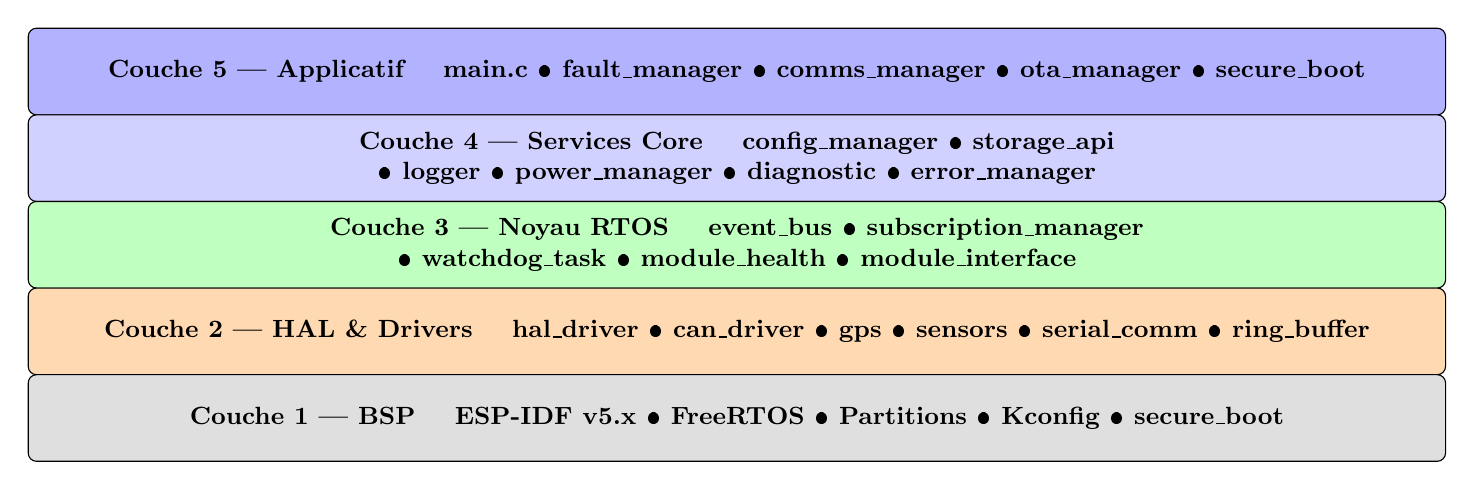
\begin{tikzpicture}[font=\small]
      \def\lw{18}
      \def\lh{1.1}
      % Couche 5
      \draw[fill=blue!30, rounded corners=3pt]
            (0,4*\lh) rectangle (\lw,5*\lh);
      \node[text width=17.5cm, align=center, font=\bfseries\small]
            at (\lw/2,4.5*\lh)
            {Couche 5 — Applicatif \quad
             main.c \textbullet\ fault\_manager \textbullet\ comms\_manager \textbullet\ ota\_manager \textbullet\ secure\_boot};
      % Couche 4
      \draw[fill=blue!18, rounded corners=3pt]
            (0,3*\lh) rectangle (\lw,4*\lh);
      \node[text width=17.5cm, align=center, font=\bfseries\small]
            at (\lw/2,3.5*\lh)
            {Couche 4 — Services Core \quad
             config\_manager \textbullet\ storage\_api \textbullet\ logger \textbullet\ power\_manager \textbullet\ diagnostic \textbullet\ error\_manager};
      % Couche 3
      \draw[fill=green!25, rounded corners=3pt]
            (0,2*\lh) rectangle (\lw,3*\lh);
      \node[text width=17.5cm, align=center, font=\bfseries\small]
            at (\lw/2,2.5*\lh)
            {Couche 3 — Noyau RTOS \quad
             event\_bus \textbullet\ subscription\_manager \textbullet\ watchdog\_task \textbullet\ module\_health \textbullet\ module\_interface};
      % Couche 2
      \draw[fill=orange!30, rounded corners=3pt]
            (0,\lh) rectangle (\lw,2*\lh);
      \node[text width=17.5cm, align=center, font=\bfseries\small]
            at (\lw/2,1.5*\lh)
            {Couche 2 — HAL \& Drivers \quad
             hal\_driver \textbullet\ can\_driver \textbullet\ gps \textbullet\ sensors \textbullet\ serial\_comm \textbullet\ ring\_buffer};
      % Couche 1
      \draw[fill=gray!25, rounded corners=3pt]
            (0,0) rectangle (\lw,\lh);
      \node[text width=17.5cm, align=center, font=\bfseries\small]
            at (\lw/2,0.5*\lh)
            {Couche 1 — BSP \quad
             ESP-IDF v5.x \textbullet\ FreeRTOS \textbullet\ Partitions \textbullet\ Kconfig \textbullet\ secure\_boot};
    \end{tikzpicture}%
    }
    \caption{Architecture logicielle en cinq couches du firmware \textit{GlobalFleet} — 23 composants ESP-IDF}
    \label{fig:archi_couches}
\end{figure}

%------------------------------------------------------------
\subsection{Main task et noyau d'exécution}
\label{subsec:main_task}
%------------------------------------------------------------

La \textit{main task}, implémentée dans \texttt{main/main.c}, est la
tâche FreeRTOS de plus haute priorité structurelle du système. Elle
est le point d'entrée unique après l'initialisation du BSP par
ESP-IDF et orchestre l'intégralité de la séquence de démarrage : elle
instancie dans l'ordre les composants de la couche~3 (event\_bus,
subscription\_manager, watchdog\_task), puis les composants de la
couche~4 (config\_manager en premier pour charger le registre de
capacités, puis les autres services core), puis les drivers de la
couche~2 conditionnellement selon le registre, et enfin les composants
applicatifs de la couche~5. Elle pilote ensuite la FSM système en
s'abonnant aux événements de transition via le \texttt{subscription\_manager}
et en invoquant les handlers d'état correspondants. Les autres tâches
FreeRTOS démarrées par les composants rapportent périodiquement leur
état au \texttt{watchdog\_task} via des heartbeats. En l'absence de
heartbeat pendant plus du timeout configuré (paramètre \texttt{wdt\_timeout\_ms}
dans \texttt{nvs\_field}), le \texttt{watchdog\_task} déclare la tâche
en défaillance et publie \texttt{EVT\_WDT\_TIMEOUT} sur le bus,
déclenchant la politique de récupération du \texttt{fault\_manager}
selon la sévérité classifiée.

%------------------------------------------------------------
\subsection{Event Bus et Subscription Manager}
\label{subsec:event_bus}
%------------------------------------------------------------

Le bus d'événements, implémenté dans le composant \texttt{event\_bus},
est le mécanisme de communication inter-modules central du firmware,
incarnant le patron \textit{Publish-Subscribe}. Il repose sur une
file FreeRTOS (\texttt{QueueHandle\_t}) et une tâche Dispatcher
dédiée qui lit séquentiellement les événements et appelle les
callbacks des abonnés enregistrés dans le \texttt{subscription\_manager}.
Les producteurs publient des événements typés (structures C de taille
fixe incluant le type d'événement et un payload union) via l'API
\texttt{event\_bus\_publish()} depuis n'importe quelle tâche ou
contexte d'interruption (via le mécanisme ISR-safe de FreeRTOS).
Les consommateurs s'abonnent via \texttt{event\_bus\_subscribe(type, callback)}
lors de leur initialisation. Ce découplage total permet d'ajouter,
de supprimer ou de remplacer un composant sans impacter les autres :
les tests hors-cible du répertoire \texttt{test\_host/} en tirent
parti en substituant les callbacks réels par des mocks Python via
\texttt{test\_subscription.py}, validant le comportement du bus sans
matériel physique. Le fichier \texttt{test/test\_subscription\_manager.c}
valide quant à lui le comportement du \texttt{subscription\_manager}
directement sur la cible ESP32-P4.
\begin{figure}[H]
    \centering
    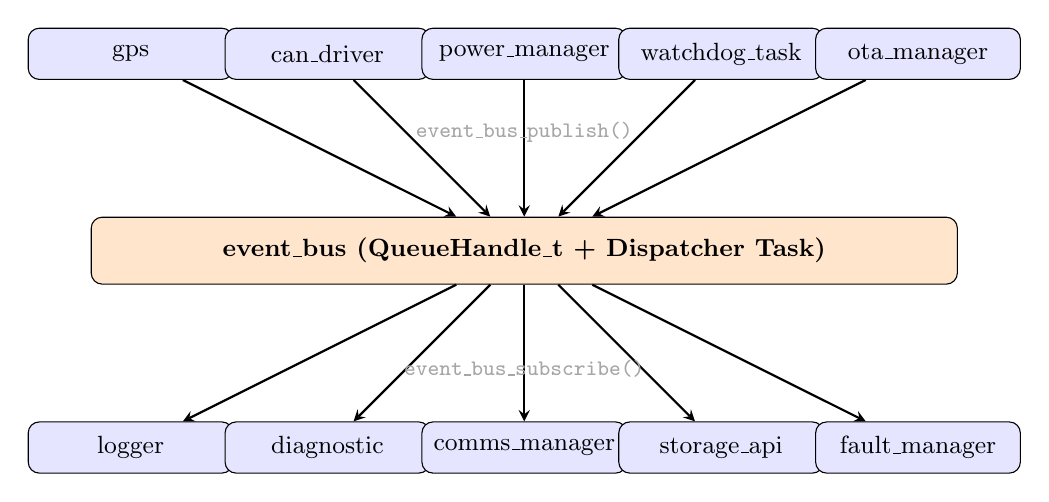
\begin{tikzpicture}[font=\small, node distance=1.4cm,
        box/.style={draw, rounded corners=4pt, minimum width=2.6cm,
                    minimum height=0.65cm, align=center, fill=blue!10},
        bus/.style={draw, rounded corners=4pt, minimum width=11cm,
                    minimum height=0.85cm, align=center, fill=orange!20,
                    font=\bfseries\small}]
      % Bus central
      \node[bus] (bus) at (5.5,0)
            {event\_bus (QueueHandle\_t + Dispatcher Task)};
      % Producteurs haut
      \node[box] (gps)    at (0.5,  2.5) {gps};
      \node[box] (can)    at (3.0,  2.5) {can\_driver};
      \node[box] (power)  at (5.5,  2.5) {power\_manager};
      \node[box] (wdt)    at (8.0,  2.5) {watchdog\_task};
      \node[box] (ota)    at (10.5, 2.5) {ota\_manager};
      % Consommateurs bas
      \node[box] (logger) at (0.5,  -2.5) {logger};
      \node[box] (diag)   at (3.0,  -2.5) {diagnostic};
      \node[box] (comms)  at (5.5,  -2.5) {comms\_manager};
      \node[box] (store)  at (8.0,  -2.5) {storage\_api};
      \node[box] (fault)  at (10.5, -2.5) {fault\_manager};
      % Flèches publish
      \foreach \n in {gps,can,power,wdt,ota}
        \draw[->, thick, >=stealth] (\n) -- (bus);
      % Flèches subscribe
      \foreach \n in {logger,diag,comms,store,fault}
        \draw[->, thick, >=stealth] (bus) -- (\n);
      % Labels
      \node[font=\footnotesize, color=gray!70] at (5.5,1.5)
            {\texttt{event\_bus\_publish()}};
      \node[font=\footnotesize, color=gray!70] at (5.5,-1.5)
            {\texttt{event\_bus\_subscribe()}};
    \end{tikzpicture}
    \caption{Architecture de l'\texttt{event\_bus} — patron Publish-Subscribe sur 10 composants}
    \label{fig:ann_event_bus}
\end{figure}

%------------------------------------------------------------
\subsection{Watchdog Task et Module Health}
\label{subsec:timers}
%------------------------------------------------------------

La supervision du comportement en temps réel de chaque tâche FreeRTOS
est assurée par deux composants complémentaires : \texttt{watchdog\_task}
et \texttt{module\_health}. Le composant \texttt{watchdog\_task}
implémente un watchdog logiciel multi-tâches : chaque tâche active
s'enregistre auprès du watchdog au démarrage et doit envoyer un
heartbeat périodique (appel à \texttt{wdt\_kick(task\_id)}) selon
une période inférieure au timeout configuré. Si une tâche omet son
heartbeat — indiquant un blocage sur une ressource, une boucle
infinie, ou un crash silencieux — \texttt{watchdog\_task} publie
\texttt{EVT\_WDT\_TIMEOUT} sur l'event bus avec l'identifiant de la
tâche fautive en payload, déclenchant la politique de récupération
du \texttt{fault\_manager}. Le composant \texttt{module\_health}
maintient en complément des compteurs de santé par module :
chaque appel à \texttt{module\_health\_report\_error(module\_id)}
incrémente le compteur correspondant, et un timer logiciel FreeRTOS
le décrémente périodiquement. Lorsque le compteur dépasse le seuil
configurable \texttt{health\_threshold}, le module est redémarré
via son interface \texttt{module\_stop()} / \texttt{module\_start()}.
Ce mécanisme graduel détecte les dégradations progressives avant
qu'elles ne provoquent un watchdog timeout, réduisant le nombre
de redémarrages complets en production.

%------------------------------------------------------------
\subsection{Interface standard des modules}
\label{subsec:module_iface}
%------------------------------------------------------------

La cohérence du cycle de vie de l'ensemble des composants est garantie
par l'interface \texttt{module\_interface\_t} définie dans le composant
\texttt{module\_interface}. Cette structure de pointeurs de fonctions
impose quatre points d'entrée obligatoires à chaque composant qui
souhaite être géré par le noyau. La fonction \texttt{module\_init()}
initialise les ressources internes du composant et enregistre ses
abonnements sur l'event bus via \texttt{event\_bus\_subscribe()}.
La fonction \texttt{module\_start()} crée et démarre la tâche FreeRTOS
associée via \texttt{xTaskCreate()}, en spécifiant la pile et la
priorité dimensionnées dans les constantes du composant. La fonction
\texttt{module\_stop()} arrête proprement la tâche, libère les
ressources allouées et désabonne les callbacks du bus, garantissant
l'absence de fuite mémoire lors des redémarrages partiels gérés par
le \texttt{fault\_manager}. La fonction \texttt{module\_handle\_event(event*)}
est le callback appelé par le Dispatcher de l'\texttt{event\_bus}
pour chaque événement souscrit. Cette interface uniforme permet à la
\textit{main task} de démarrer, arrêter et redémarrer n'importe quel
composant via un tableau de pointeurs \texttt{module\_interface\_t},
sans connaissance de l'implémentation concrète.

%------------------------------------------------------------
\subsection{Fault Manager}
\label{subsec:inter_modules}
%------------------------------------------------------------

Le composant \texttt{fault\_manager} centralise la logique de
détection, classification et récupération des fautes système. Il
s'abonne aux événements \texttt{EVT\_WDT\_TIMEOUT},
\texttt{EVT\_FAULT\_DETECTED} et \texttt{EVT\_FAULT\_CRITICAL} sur
l'event bus, et maintient un catalogue interne de codes d'erreurs
typés couvrant l'ensemble des composants du firmware. À la réception
d'une faute, il consulte la table de politique (tableau~\ref{tab:fault_policy})
et applique l'action correspondante : journalisation via \texttt{logger},
redémarrage du module fautif avec backoff exponentiel (1s, 2s, 4s, 8s)
via l'interface \texttt{module\_interface\_t}, ou redémarrage complet
du système. Le mécanisme anti-boucle maintient un compteur de
redémarrages dans une fenêtre glissante de 60~secondes persistée
en NVS pour résister aux coupures d'alimentation : si ce compteur
dépasse trois, la faute est reclassifiée \texttt{FATAL} et le
\texttt{fault\_manager} active le mode safe minimal en arrêtant
tous les composants non essentiels. Un snapshot complet de l'état
système (raison de faute, heap libre, watermarks de pile, historique
des dix derniers événements du bus) est persisté en NVS par le
composant \texttt{diagnostic} et transmis au serveur via
\texttt{comms\_manager} lors du rétablissement de la connectivité.

%============================================================
\section{Architecture des services core}
\label{sec:services_core}
%============================================================

%------------------------------------------------------------
\subsection{Module Config Manager}
\label{subsec:mod_config}
%------------------------------------------------------------

Le composant \texttt{config\_manager} est le premier service core
initialisé dans la séquence de démarrage de la \textit{main task},
car tous les autres composants dépendent de ses paramètres pour
configurer leur comportement. Il gère la lecture, l'écriture et la
validation des paramètres système en deux catégories distinctes,
respectivement persistées dans les partitions NVS \texttt{nvs\_factory}
et \texttt{nvs\_field} déclarées dans \texttt{partitions.csv}. La
configuration factory (identifiant du dispositif, type de matériel,
valeur du registre de capacités, clés TLS) est lue au démarrage et
mise en cache en mémoire pour les accès ultérieurs sans I/O NVS.
La configuration field (APN, broker MQTT, intervalles de reporting,
seuils de détection) est lue depuis \texttt{nvs\_field} après
vérification CRC-32 et comparaison de numéro de version. L'API
exposée comprend \texttt{config\_get(key, value)},
\texttt{config\_set(key, value)} et \texttt{config\_apply()} qui
persiste les modifications validées et publie \texttt{EVT\_CONFIG\_CHANGED}
sur l'event bus. 
\newpage 
Toute tentative de modification d'une clé factory
est rejetée par vérification du drapeau \texttt{factory\_locked}.

\begin{figure}[H]
    \centering
    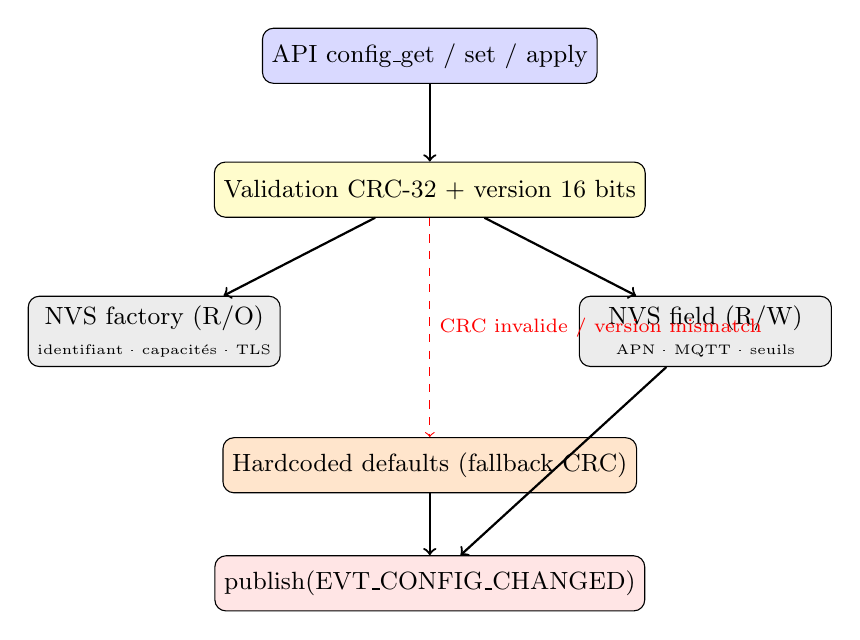
\begin{tikzpicture}[font=\small, node distance=1.8cm,
        box/.style={draw, rounded corners=4pt, minimum width=3.4cm,
                    minimum height=0.7cm, align=center},
        nvs/.style={draw, rounded corners=4pt, minimum width=3.2cm,
                    minimum height=0.7cm, align=center, fill=gray!15}]
      \node[box, fill=blue!15]   (api)     at (0,0)     {API config\_get / set / apply};
      \node[box, fill=yellow!20] (valid)   at (0,-1.7)  {Validation CRC-32 + version 16 bits};
      \node[nvs]                 (factory) at (-3.5,-3.5){NVS factory (R/O)\\{\tiny identifiant · capacités · TLS}};
      \node[nvs]                 (field)   at (3.5,-3.5) {NVS field (R/W)\\{\tiny APN · MQTT · seuils}};
      \node[box, fill=orange!20] (fallback)at (0,-5.2)  {Hardcoded defaults (fallback CRC)};
      \node[box, fill=red!10]    (pub)     at (0,-6.7)  {publish(EVT\_CONFIG\_CHANGED)};
      \draw[->, thick] (api)      -- (valid);
      \draw[->, thick] (valid)    -- (factory);
      \draw[->, thick] (valid)    -- (field);
      \draw[->, dashed, red] (valid)  --
            node[right, font=\scriptsize]{CRC invalide / version mismatch}
            (fallback);
      \draw[->, thick] (field)    -- (pub);
      \draw[->, thick] (fallback) -- (pub);
    \end{tikzpicture}
    \caption{Architecture du composant \texttt{config\_manager} — double partition NVS, validation et fallback}
    \label{fig:config_module}
\end{figure}

%------------------------------------------------------------
\subsection{Module Storage API}
\label{subsec:mod_storage}
%------------------------------------------------------------

Le composant \texttt{storage\_api} abstrait l'accès au système de
fichiers embarqué (SPIFFS ou LittleFS selon la configuration Kconfig)
et à la mémoire flash NVS pour les données applicatives. Il gère
trois partitions logiques : \texttt{log} pour les journaux de
\texttt{logger}, \texttt{config} pour les sauvegardes de
\texttt{config\_manager}, et \texttt{offline\_data} pour les
données télématiques accumulées en l'absence de connectivité.
Le composant \texttt{ring\_buffer}, utilisé en interne par
\texttt{storage\_api}, implémente un ring buffer en mémoire RAM qui
amortit les écritures flash et préserve l'endurance de la mémoire
en regroupant les petites écritures en blocs de taille optimale pour
le matériel flash sous-jacent. En cas d'absence de connectivité,
les trames GPS et CAN sont sérialisées et stockées dans
\texttt{offline\_data} ; lors du rétablissement, la réception de
l'événement \texttt{EVT\_COMMS\_CONNECTED} par le \texttt{storage\_api}
déclenche l'envoi différé des données par ordre chronologique via
\texttt{comms\_manager}, garantissant la complétude des traces
télémétriques. Le composant surveille le taux de remplissage de
chaque partition et publie \texttt{EVT\_STORAGE\_FULL} lorsque
le seuil configuré est atteint, permettant au \texttt{power\_manager}
d'adapter la fréquence de reporting.

%------------------------------------------------------------
\subsection{Module Logger}
\label{subsec:mod_logger}
%------------------------------------------------------------

Le composant \texttt{logger} collecte et persiste les messages de
journalisation de l'ensemble des composants du firmware de manière
structurée et horodatée. Il supporte quatre niveaux de sévérité :
\texttt{DEBUG} pour les traces de développement désactivées en
production via Kconfig, \texttt{INFO} pour les événements nominaux,
\texttt{WARNING} pour les anomalies récupérables, et \texttt{ERROR}
pour les défaillances nécessitant intervention. Chaque entrée de log
est produite au format JSON structuré, incluant l'horodatage RTC
synchronisé GNSS (fourni par le composant \texttt{gps}), le nom
du composant émetteur, le niveau de sévérité, et un champ message
libre. Ces entrées sont d'abord stockées dans le ring buffer RAM
géré par le composant \texttt{ring\_buffer} pour les accès fréquents,
puis purgées périodiquement vers la partition Flash \texttt{log} via
\texttt{storage\_api} selon la politique de rotation configurée
(taille maximale de fichier, nombre de fichiers rotatifs). En cas
d'erreur critique, le \texttt{logger} est invoqué directement par
le \texttt{fault\_manager} pour garantir la persistance immédiate
du journal avant redémarrage. Un mécanisme de dump via UART, géré
par le composant \texttt{serial\_comm} et le driver \texttt{hal\_uart},
permet l'extraction des logs pour débogage sur le terrain sans
démontage de l'appareil.

%------------------------------------------------------------
\subsection{Module Power Manager}
\label{subsec:mod_power}
%------------------------------------------------------------

Le composant \texttt{power\_manager} contrôle les transitions entre
quatre modes d'alimentation selon des règles opérationnelles
configurées dans la partition \texttt{nvs\_field}. En mode
\textbf{ACTIVE}, tous les périphériques sont alimentés et toutes
les tâches actives : la consommation typique est de 40~mA pour la
variante Basic, 80~mA pour la variante Pro, et 120~mA pour
Ultra-Pro en raison des modules CAN-FD et sécurité additionnels.
En mode \textbf{REDUCED}, le module cellulaire passe en PSM LTE
Cat-M1 (Power Saving Mode) et le composant \texttt{gps} réduit
sa fréquence de fix. En mode \textbf{SLEEP}, le \texttt{power\_manager}
désactive via les sorties GPIO (\texttt{hal\_gpio}) les alimentations
des périphériques non essentiels (module cellulaire, GPS, CAN) et
met le cœur principal ESP32-P4 en veille légère, laissant seul le
coprocesseur LP actif pour la surveillance des sources de réveil.
En mode \textbf{DEEP\_SLEEP} (Ultra-Pro uniquement, nécessitant le
bit 5 du registre de capacités), tous les domaines HP sont coupés
pour atteindre une consommation inférieure à 2~mA, suffisante pour
les appareils alimentés uniquement sur batterie de secours.
Le \texttt{power\_manager} publie \texttt{EVT\_POWER\_SLEEP} et
\texttt{EVT\_POWER\_WAKE} pour notifier les autres composants et
leur permettre de persister leur état avant extinction.

%------------------------------------------------------------
\subsection{Module Diagnostic}
\label{subsec:mod_diag}
%------------------------------------------------------------

Le composant \texttt{diagnostic} maintient un tableau de bord système
en temps réel, exposant l'état de santé global de l'appareil au
serveur de gestion de flotte. Il collecte et agrège en permanence
les métriques suivantes : la raison du dernier redémarrage
(\textit{reset reason}) lue depuis les registres ESP32 au démarrage,
le temps de fonctionnement cumulé depuis la mise en service
(\textit{uptime}), l'état de santé et les health counters de chaque
composant fournis par \texttt{module\_health}, l'utilisation mémoire
(heap libre, watermark de pile par tâche FreeRTOS), et les
statistiques réseau (pertes MQTT, délais de transmission, nombre de
reconnexions) fournies par \texttt{comms\_manager}. Ces métriques
sont sérialisées au format JSON et transmises périodiquement au
serveur via un topic MQTT dédié \texttt{sat/<device\_id>/diagnostic}.
Lors d'une transition vers l'état \texttt{FAULT}, le \texttt{diagnostic}
est invoqué par le \texttt{fault\_manager} pour persister un snapshot
complet en NVS avant redémarrage, incluant les dix derniers événements
de l'event bus, garantissant un diagnostic post-mortem précis sans
accès physique à l'appareil après récupération de la connectivité.

%------------------------------------------------------------
\subsection{Module Error Manager}
\label{subsec:mod_error}
%------------------------------------------------------------

Le composant \texttt{error\_manager} centralise la gestion des erreurs
déclarées par les autres composants via l'API
\texttt{error\_report(module\_id, error\_code, severity)}. Il maintient
un catalogue de codes d'erreurs typés couvrant l'ensemble des domaines
du firmware : erreurs driver (codes 0x1000--0x1FFF), erreurs NVS
(0x2000--0x2FFF), erreurs réseau (0x3000--0x3FFF), erreurs FOTA
(0x4000--0x4FFF). À la réception d'un rapport d'erreur, il consulte
la table de politique du tableau~\ref{tab:fault_policy} et applique
l'action correspondante : simple journalisation via \texttt{logger}
pour un \texttt{WARNING}, redémarrage du composant fautif avec backoff
exponentiel (1s, 2s, 4s, 8s) pour un \texttt{ERROR}, ou transition
vers l'état \texttt{FAULT} de la FSM via publication de
\texttt{EVT\_FAULT\_CRITICAL} pour un \texttt{CRITICAL}. Le mécanisme
de backoff exponentiel est essentiel pour éviter les redémarrages en
boucle lors d'erreurs persistantes (driver matériel défaillant,
ressource externe indisponible) : il laisse le temps au système de
se stabiliser entre deux tentatives. Le mécanisme anti-boucle
surveille le nombre de redémarrages dans une fenêtre glissante de
60~secondes persistée en NVS et reclassifie toute faute en
\texttt{FATAL} au-delà de trois occurrences.

%============================================================
\section{Architecture HAL et extensibilité}
\label{sec:hal}
%============================================================

%------------------------------------------------------------
\subsection{Rôle de la HAL}
\label{subsec:hal_role}
%------------------------------------------------------------

La couche d'abstraction matérielle (HAL), implémentée dans le composant
\texttt{hal\_driver}, isole les services applicatifs des détails
d'implémentation des périphériques physiques de l'ESP32-P4. Elle
définit des interfaces C stables sous la forme de structures de
pointeurs de fonctions — \texttt{hal\_gpio\_t} dans \texttt{hal\_gpio.h}
et \texttt{hal\_uart\_t} dans \texttt{hal\_uart.h} — qui permettent
de substituer un driver matériel par un stub de test sans modifier
le code applicatif. Les fichiers d'implémentation correspondants
(\texttt{hal\_gpio.c} et \texttt{hal\_uart.c}) contiennent les appels
aux primitives ESP-IDF bas niveau (\texttt{gpio\_set\_direction()},
\texttt{uart\_driver\_install()}, etc.), strictement isolés de la
logique applicatif. Chaque driver respecte une structure standardisée
à quatre opérations cohérente avec l'interface
\texttt{module\_interface\_t} : \texttt{drv\_init()} pour
l'initialisation et la configuration des périphériques, \texttt{drv\_read()}
pour la lecture de données, \texttt{drv\_write()} pour l'écriture,
et \texttt{drv\_deinit()} pour la libération propre des ressources.
Cette interface stable est essentielle pour la portabilité du firmware
sur d'autres microcontrôleurs de la famille ESP32, envisagée dans
les perspectives d'évolution du projet.

\begin{figure}[H]
\centering
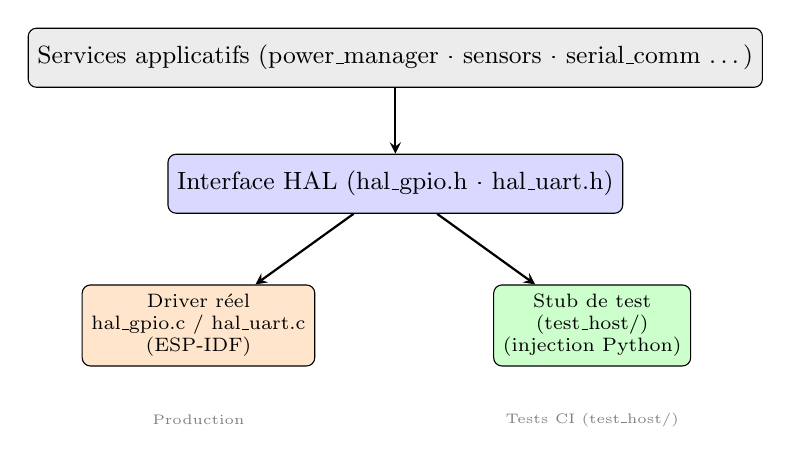
\begin{tikzpicture}[font=\small,
  layer/.style={draw, rounded corners=3pt, minimum width=5.5cm,
                minimum height=0.75cm, align=center, fill=#1},
  impl/.style={draw, rounded corners=3pt, minimum width=2.4cm,
               minimum height=0.65cm, align=center, fill=#1, font=\scriptsize},
  arr/.style={<->, thick, >=stealth, dashed}
]
  % Interface HAL (contrat)
  \node[layer=blue!15]   (ihal)  at (0, 0)    {Interface HAL (hal\_gpio.h · hal\_uart.h)};
  % Deux implémentations
  \node[impl=orange!20]  (real)  at (-2.5,-1.8) {Driver réel\\hal\_gpio.c / hal\_uart.c\\(ESP-IDF)};
  \node[impl=green!20]   (stub)  at ( 2.5,-1.8) {Stub de test\\(test\_host/)\\(injection Python)};
  % Services applicatifs au-dessus
  \node[layer=gray!15]   (svc)   at (0, 1.6)
        {Services applicatifs (power\_manager · sensors · serial\_comm …)};
  % Flèches
  \draw[->, thick, >=stealth] (svc)  -- (ihal);
  \draw[->, thick, >=stealth] (ihal) -- (real);
  \draw[->, thick, >=stealth] (ihal) -- (stub);
  \node[font=\tiny, gray] at (-2.5,-3.0) {Production};
  \node[font=\tiny, gray] at ( 2.5,-3.0) {Tests CI (test\_host/)};
\end{tikzpicture}
\caption{Architecture HAL — interface stable avec double implémentation réelle et stub de test}
\label{fig:hal_archi}
\end{figure}

%------------------------------------------------------------
\subsection{Drivers HAL implémentés : GPIO et UART}
\label{subsec:hal_ajout}
%------------------------------------------------------------

Le composant \texttt{hal\_driver} livre deux drivers physiques
complets : \texttt{hal\_gpio} et \texttt{hal\_uart}. Le driver
\texttt{hal\_gpio} gère les entrées/sorties numériques de l'ESP32-P4 :
configuration de la direction (entrée/sortie), lecture d'état,
écriture de niveau logique, et configuration des interruptions GPIO
pour les sources de réveil du \texttt{power\_manager}. Il est utilisé
par le \texttt{power\_manager} pour piloter les lignes d'activation
des alimentations périphériques (module cellulaire, GPS, CAN) et par
le composant \texttt{sensors} pour lire les capteurs numériques
additionnels de la variante Pro. Le driver \texttt{hal\_uart}
gère la communication série asynchrone : configuration du débit
(\textit{baud rate}), de la taille de trame et de la parité via
l'API ESP-IDF \texttt{uart\_driver\_install()}, émission et réception
avec buffers DMA pour minimiser la charge CPU. Il est utilisé par le
composant \texttt{serial\_comm} pour la communication locale de
diagnostic et de configuration de premier démarrage, et par le
composant \texttt{gps} pour la réception des trames NMEA ou UBX
du module GNSS connecté en UART. L'intégration de ces deux drivers
dans le composant \texttt{hal\_driver} avec leurs fichiers
\texttt{CMakeLists.txt} dédiés illustre concrètement la règle d'ajout
de périphérique qui peut être généralisée à tout nouveau capteur.

%------------------------------------------------------------
\subsection{Règles d'ajout d'un nouveau périphérique}
\label{subsec:hal_stubs}
%------------------------------------------------------------

L'intégration d'un nouveau périphérique dans le firmware
\textit{GlobalFleet} suit un protocole en quatre étapes documenté
et reproductible. Premièrement, définir la structure d'interface HAL
dans un nouveau fichier \texttt{hal\_<periph>.h} dans le répertoire
\texttt{hal\_driver/include} en exposant les quatre opérations
standardisées (\texttt{init}, \texttt{read}, \texttt{write},
\texttt{deinit}). Deuxièmement, implémenter le driver dans
\texttt{hal\_driver/src/hal\_<periph>.c} en s'appuyant uniquement
sur les primitives ESP-IDF, sans référencer aucun service applicatif.
Troisièmement, enregistrer le bit de capacité correspondant dans le
registre 32~bits du \texttt{config\_manager} et déclarer la
fonctionnalité dans le tableau des variantes. Quatrièmement, ajouter
un stub de test dans le répertoire \texttt{test\_host/} implémentant
la même interface avec des données simulées injectables par les
scripts Python (\texttt{test\_subscription.py},
\texttt{mqtt\_test.py}), permettant une validation complète du
comportement applicatif sans matériel physique via l'infrastructure
CI. Cette procédure garantit que chaque nouveau périphérique est
immédiatement testable, configurable par variante et documenté dans
le registre de capacités.

%------------------------------------------------------------
\subsection{Séparation entre drivers physiques et services applicatifs}
\label{subsec:hal_sep}
%------------------------------------------------------------

La règle de séparation entre la couche HAL et les services applicatifs
est strictement appliquée dans l'organisation du dépôt
\textit{GlobalFleet}. Les drivers HAL (\texttt{hal\_gpio.c},
\texttt{hal\_uart.c}) ne contiennent que la communication bas niveau
avec les périphériques physiques : lecture de registres, gestion des
interruptions, configuration DMA, et respect des timings matériels.
Toute logique métier réside dans les services applicatifs de la
couche~4 : le filtrage et la validation des trames GNSS sont gérés
par le composant \texttt{gps}, l'agrégation et le décodage des trames
CAN J1939 par le composant \texttt{can\_driver} à la couche~2 mais
avec son propre composant de traitement, et la gestion des alertes
sur les capteurs par le composant \texttt{sensors}. Cette séparation
rend les drivers testables en isolation totale via les stubs du
\texttt{test\_host/}, réutilisables sur d'autres projets de la
gamme SAT partageant le même matériel ESP32-P4, et remplaçables
sans aucun impact sur le code métier. Elle facilite également la
certification du code : la couche HAL, de surface réduite et sans
logique métier, peut être soumise à une revue de code ciblée sur
la conformité aux spécifications matérielles de l'ESP32-P4.

%============================================================
\section{Architecture communication}
\label{sec:comms}
%============================================================

%------------------------------------------------------------
\subsection{Interface CommsProvider}
\label{subsec:comms_iface}
%------------------------------------------------------------

L'interface \texttt{CommsProvider}, définie dans le composant
\texttt{comms\_provider}, constitue l'abstraction centrale de la
couche de communication du firmware. Elle expose quatre primitives
indépendantes du protocole sous-jacent : \texttt{connect(host, port)}
pour l'établissement de la connexion, \texttt{disconnect()} pour
la fermeture propre, \texttt{publish(topic, payload, qos)} pour
l'émission de données vers le serveur, et \texttt{subscribe(topic, callback)}
pour la réception de commandes. Cette interface C, implémentée comme
une structure de pointeurs de fonctions (patron \textit{Strategy}
en langage C), permet de changer de protocole de transport sans
modifier une seule ligne du code des composants producteurs de données.
Les composants \texttt{gps}, \texttt{can\_driver}, \texttt{sensors}
et \texttt{diagnostic} publient leurs données via \texttt{comms\_provider}
sans connaître le protocole actif. Le composant \texttt{comms\_manager}
orchestre l'utilisation de cette interface : il instancie
l'implémentation concrète selon la configuration terrain, gère la
reconnexion automatique avec stratégie de backoff exponentiel (1s,
2s, 4s, 8s) en cas de perte de connectivité, et publie
\texttt{EVT\_COMMS\_CONNECTED} ou \texttt{EVT\_COMMS\_LOST} sur
l'event bus pour notifier les autres composants.

%------------------------------------------------------------
\subsection{Comms Manager et sélecteur runtime du protocole}
\label{subsec:comms_sel}
%------------------------------------------------------------

Le protocole de communication actif est sélectionné à l'exécution
par le composant \texttt{comms\_manager}, qui lit le champ
\texttt{cfg.comms.protocol} depuis \texttt{config\_manager} lors de
son initialisation. Trois protocoles sont supportés : MQTT via
TLS~1.3 (recommandé pour les variantes Pro et Ultra-Pro), TCP brut
avec TLS~1.3 optionnel, et UDP sans garantie de livraison pour les
trames haute fréquence de faible priorité. La sélection instancie
l'implémentation concrète de \texttt{CommsProvider} correspondante
via une table de pointeurs de fonctions indexée par l'identifiant
de protocole — mécanisme équivalent au patron \textit{Strategy}
de la littérature orientée objet, implémenté en C pur sans surcoût
de vtable.

Concrètement, la table \texttt{comms\_provider\_table[]} associe à
chaque identifiant de protocole (\texttt{COMMS\_MQTT},
\texttt{COMMS\_TCP}, \texttt{COMMS\_UDP}) une structure
\texttt{comms\_provider\_t} renseignant les quatre pointeurs de
fonctions \texttt{connect}, \texttt{disconnect}, \texttt{publish} et
\texttt{subscribe}. Au démarrage, \texttt{comms\_manager} recopie
simplement le pointeur correspondant au protocole configuré dans une
variable globale \texttt{active\_provider}, qui sera utilisée par
tous les appels ultérieurs sans branchement conditionnel
(\texttt{if}/\texttt{switch}) dans le reste du code. Ce choix garantit
un temps d'accès constant et déterministe, compatible avec les
contraintes temps réel imposées par FreeRTOS.

Au-delà de la sélection initiale, \texttt{comms\_manager} encapsule
également la logique de supervision de la connexion : une tâche
dédiée surveille périodiquement l'état du lien via
\texttt{active\_provider->connect()}, et déclenche, en cas
d'échec, une stratégie de reconnexion par backoff exponentiel
(1\,s, 2\,s, 4\,s, 8\,s) avant de republier
\texttt{EVT\_COMMS\_LOST} sur l'\texttt{event\_bus}. Lors du
rétablissement, \texttt{EVT\_COMMS\_CONNECTED} est publié,
permettant au \texttt{storage\_api} de déclencher l'envoi différé
des données accumulées en mode \textit{offline}. Cette séparation
stricte entre la logique de sélection/supervision, portée par
\texttt{comms\_manager}, et l'implémentation bas niveau de chaque
protocole, portée par \texttt{comms\_provider}, permet d'ajouter de
nouveaux protocoles de transport (LoRaWAN, LwM2M, CoAP envisagés
dans les perspectives) 
\newpage en créant simplement une nouvelle
implémentation de l'interface \texttt{CommsProvider} et en
l'enregistrant dans la table, sans toucher au code des composants
producteurs de données ni à celui du \texttt{comms\_manager}
lui-même.

\begin{figure}[H]
\centering
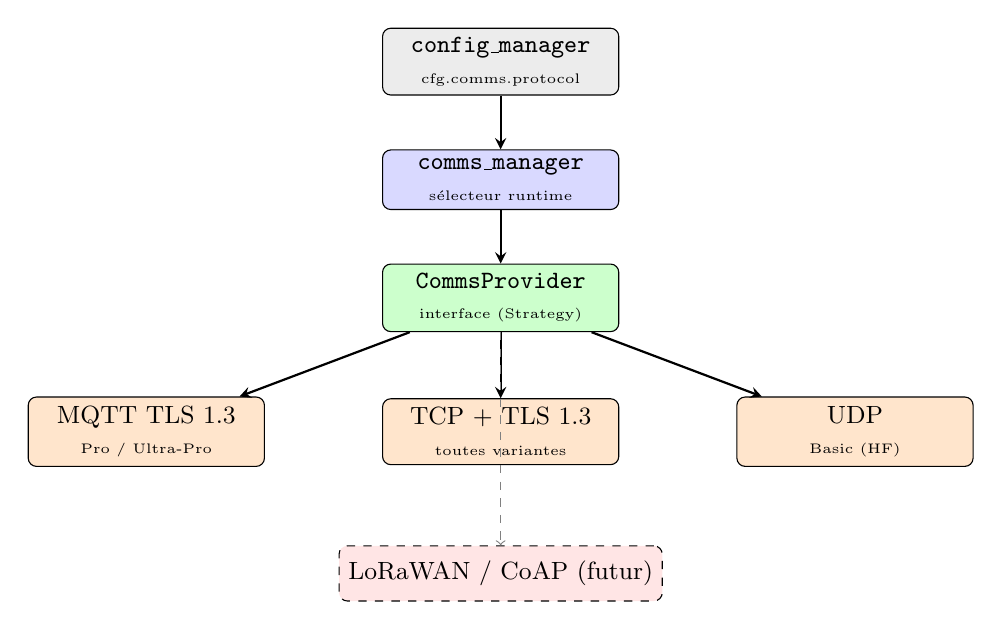
\begin{tikzpicture}[font=\small,
  box/.style={draw, rounded corners=3pt, minimum width=3.0cm,
              minimum height=0.7cm, align=center, fill=#1},
  arr/.style={->, thick, >=stealth}
]
  \node[box=gray!15]  (cfg)  at (0, 3.5)   {\texttt{config\_manager}\\{\tiny cfg.comms.protocol}};
  \node[box=blue!15]  (cm)   at (0, 2.0)   {\texttt{comms\_manager}\\{\tiny sélecteur runtime}};
  \node[box=green!20] (iface)at (0, 0.5)   {\texttt{CommsProvider}\\{\tiny interface (Strategy)}};
  \node[box=orange!20](mqtt) at (-4.5,-1.2){MQTT TLS 1.3\\{\tiny Pro / Ultra-Pro}};
  \node[box=orange!20](tcp)  at (0,   -1.2){TCP + TLS 1.3\\{\tiny toutes variantes}};
  \node[box=orange!20](udp)  at (4.5, -1.2){UDP\\{\tiny Basic (HF)}};
  \draw[arr] (cfg)   -- (cm);
  \draw[arr] (cm)    -- (iface);
  \draw[arr] (iface) -- (mqtt);
  \draw[arr] (iface) -- (tcp);
  \draw[arr] (iface) -- (udp);
  % Futurs
  \node[box=red!10, dashed] (lora) at (0,-3.0)
        {LoRaWAN / CoAP (futur)};
  \draw[->, dashed, gray] (iface) -- (lora);
\end{tikzpicture}
\caption{Sélecteur runtime du protocole — patron Strategy via \texttt{comms\_provider}}
\label{fig:comms_strategy}
\end{figure}

%------------------------------------------------------------
\subsection{Configuration TCP, UDP et MQTT}
\label{subsec:comms_config}
%------------------------------------------------------------

Chaque protocole dispose de ses propres paramètres dans la partition
\texttt{nvs\_field} gérée par \texttt{config\_manager} : adresse et
port du serveur distant, topic racine MQTT structuré selon la
convention \texttt{sat/<device\_id>/<data\_type>} (ex.
\texttt{sat/SAT-0042/gps}, \texttt{sat/SAT-0042/can},
\texttt{sat/SAT-0042/diagnostic}), QoS MQTT configurable (0 pour les
trames GPS haute fréquence, 1 pour les alertes, 2 pour les données
de diagnostic critiques) selon la criticité du message, timeout de
connexion et taille maximale des messages en octets. La sécurité des
communications est assurée par TLS~1.3 pour les protocoles TCP et
MQTT, avec vérification du certificat serveur via un magasin de
certificats (CA bundle) stocké dans une partition Flash dédiée,
protégée par Flash Encryption en variante Ultra-Pro. Le certificat
client est stocké dans la partition NVS factory lors de la
programmation usine, garantissant l'authentification mutuelle entre
l'appareil et le serveur de gestion de flotte. Ces paramètres sont
modifiables à distance via une commande MQTT dédiée reçue sur le topic
\texttt{sat/<device\_id>/cmd/config}, traitée par le
\texttt{comms\_manager} et répercutée sur \texttt{config\_manager}.

%------------------------------------------------------------
\subsection{Serial Comm et communication locale}
\label{subsec:comms_mocks}
%------------------------------------------------------------

Le composant \texttt{serial\_comm}, appuyé sur le driver
\texttt{hal\_uart}, assure la communication locale par port série
pour deux cas d'usage distincts. En phase de déploiement usine, il
expose une interface de commande série permettant d'écrire la
configuration factory (\texttt{nvs\_factory}), de positionner le
registre de capacités selon le profil matériel de l'appareil, et
de valider la programmation avant mise en service. En phase de
maintenance terrain, il permet l'extraction des logs via la commande
dump invoquée par \texttt{logger}, le diagnostic en temps réel des
métriques exposées par \texttt{diagnostic}, et la mise à jour de
configuration field sans nécessiter de connectivité cellulaire.
Les tests hors-cible du répertoire \texttt{test\_host/} exploitent
indirectement ce mécanisme : les scripts Python
\texttt{test\_subscription.py} et \texttt{mqtt\_test.py} simulent
le canal de communication et injectent des événements dans l'event
bus pour valider le comportement des composants applicatifs sans
matériel physique, une approche essentielle pour l'intégration
continue du projet.

%------------------------------------------------------------
\subsection{Préparation à l'intégration d'un canal réel}
\label{subsec:comms_reel}
%------------------------------------------------------------

L'architecture de communication a été conçue dès la conception pour
faciliter l'intégration future d'un canal cellulaire réel 4G/LTE
ou de protocoles alternatifs tels que LoRaWAN, LwM2M ou CoAP,
identifiés dans les perspectives d'évolution du projet. Grâce à
l'interface \texttt{CommsProvider} abstraite, il suffit d'implémenter
les quatre primitives (\texttt{connect}, \texttt{disconnect},
\texttt{publish}, \texttt{subscribe}) pour le nouveau canal et
d'enregistrer l'implémentation dans la table de sélection du
\texttt{comms\_manager}, sans modifier le moindre composant producteur
de données. Un nouveau bit de capacité dans le registre 32~bits du
\texttt{config\_manager} contrôle l'activation du nouveau canal selon
la variante matérielle. Les données en attente de transmission sont
maintenues dans l'offline buffer de \texttt{storage\_api} via le
composant \texttt{ring\_buffer} durant toute indisponibilité du canal,
garantissant leur intégrité et leur transmission ordonnée lors du
rétablissement de la connectivité. Cette architecture garantit que
l'évolution de la pile de communication n'impacte jamais les composants
de collecte et de traitement des données télémétriques.

%============================================================
\section{Conclusion}
\label{sec:conclu_ch3}
%============================================================

Ce chapitre a posé les bases conceptuelles du firmware générique
\textit{GlobalFleet} : six besoins (généricité, modularité,
configurabilité, fiabilité, intégration cloud, fonctionnel) ont
structuré les vingt-trois composants ESP-IDF du projet selon une
architecture en cinq couches (BSP, HAL, Noyau RTOS, Services Core,
Applicatif). Le modèle de capacités — registre 32~bits NVS interrogé
via \texttt{HAS\_CAPABILITY()} — permet de couvrir les variantes
\textbf{Basic}, \textbf{Pro} et \textbf{Ultra-Pro} avec une base de
code unique. La FSM à cinq états (INIT, RUN, SLEEP, UPDATE, FAULT),
pilotée par l'\texttt{event\_bus} et le \texttt{subscription\_manager}
(dix-huit événements typés), formalise le comportement global et la
récupération graduée des fautes via \texttt{fault\_manager}. Ce socle
est implémenté et validé dans les chapitres~IV et~V.